% Options for packages loaded elsewhere
\PassOptionsToPackage{unicode}{hyperref}
\PassOptionsToPackage{hyphens}{url}
%
\documentclass[
]{book}
\usepackage{amsmath,amssymb}
\usepackage{lmodern}
\usepackage{iftex}
\ifPDFTeX
  \usepackage[T1]{fontenc}
  \usepackage[utf8]{inputenc}
  \usepackage{textcomp} % provide euro and other symbols
\else % if luatex or xetex
  \usepackage{unicode-math}
  \defaultfontfeatures{Scale=MatchLowercase}
  \defaultfontfeatures[\rmfamily]{Ligatures=TeX,Scale=1}
\fi
% Use upquote if available, for straight quotes in verbatim environments
\IfFileExists{upquote.sty}{\usepackage{upquote}}{}
\IfFileExists{microtype.sty}{% use microtype if available
  \usepackage[]{microtype}
  \UseMicrotypeSet[protrusion]{basicmath} % disable protrusion for tt fonts
}{}
\makeatletter
\@ifundefined{KOMAClassName}{% if non-KOMA class
  \IfFileExists{parskip.sty}{%
    \usepackage{parskip}
  }{% else
    \setlength{\parindent}{0pt}
    \setlength{\parskip}{6pt plus 2pt minus 1pt}}
}{% if KOMA class
  \KOMAoptions{parskip=half}}
\makeatother
\usepackage{xcolor}
\usepackage{color}
\usepackage{fancyvrb}
\newcommand{\VerbBar}{|}
\newcommand{\VERB}{\Verb[commandchars=\\\{\}]}
\DefineVerbatimEnvironment{Highlighting}{Verbatim}{commandchars=\\\{\}}
% Add ',fontsize=\small' for more characters per line
\usepackage{framed}
\definecolor{shadecolor}{RGB}{248,248,248}
\newenvironment{Shaded}{\begin{snugshade}}{\end{snugshade}}
\newcommand{\AlertTok}[1]{\textcolor[rgb]{0.94,0.16,0.16}{#1}}
\newcommand{\AnnotationTok}[1]{\textcolor[rgb]{0.56,0.35,0.01}{\textbf{\textit{#1}}}}
\newcommand{\AttributeTok}[1]{\textcolor[rgb]{0.77,0.63,0.00}{#1}}
\newcommand{\BaseNTok}[1]{\textcolor[rgb]{0.00,0.00,0.81}{#1}}
\newcommand{\BuiltInTok}[1]{#1}
\newcommand{\CharTok}[1]{\textcolor[rgb]{0.31,0.60,0.02}{#1}}
\newcommand{\CommentTok}[1]{\textcolor[rgb]{0.56,0.35,0.01}{\textit{#1}}}
\newcommand{\CommentVarTok}[1]{\textcolor[rgb]{0.56,0.35,0.01}{\textbf{\textit{#1}}}}
\newcommand{\ConstantTok}[1]{\textcolor[rgb]{0.00,0.00,0.00}{#1}}
\newcommand{\ControlFlowTok}[1]{\textcolor[rgb]{0.13,0.29,0.53}{\textbf{#1}}}
\newcommand{\DataTypeTok}[1]{\textcolor[rgb]{0.13,0.29,0.53}{#1}}
\newcommand{\DecValTok}[1]{\textcolor[rgb]{0.00,0.00,0.81}{#1}}
\newcommand{\DocumentationTok}[1]{\textcolor[rgb]{0.56,0.35,0.01}{\textbf{\textit{#1}}}}
\newcommand{\ErrorTok}[1]{\textcolor[rgb]{0.64,0.00,0.00}{\textbf{#1}}}
\newcommand{\ExtensionTok}[1]{#1}
\newcommand{\FloatTok}[1]{\textcolor[rgb]{0.00,0.00,0.81}{#1}}
\newcommand{\FunctionTok}[1]{\textcolor[rgb]{0.00,0.00,0.00}{#1}}
\newcommand{\ImportTok}[1]{#1}
\newcommand{\InformationTok}[1]{\textcolor[rgb]{0.56,0.35,0.01}{\textbf{\textit{#1}}}}
\newcommand{\KeywordTok}[1]{\textcolor[rgb]{0.13,0.29,0.53}{\textbf{#1}}}
\newcommand{\NormalTok}[1]{#1}
\newcommand{\OperatorTok}[1]{\textcolor[rgb]{0.81,0.36,0.00}{\textbf{#1}}}
\newcommand{\OtherTok}[1]{\textcolor[rgb]{0.56,0.35,0.01}{#1}}
\newcommand{\PreprocessorTok}[1]{\textcolor[rgb]{0.56,0.35,0.01}{\textit{#1}}}
\newcommand{\RegionMarkerTok}[1]{#1}
\newcommand{\SpecialCharTok}[1]{\textcolor[rgb]{0.00,0.00,0.00}{#1}}
\newcommand{\SpecialStringTok}[1]{\textcolor[rgb]{0.31,0.60,0.02}{#1}}
\newcommand{\StringTok}[1]{\textcolor[rgb]{0.31,0.60,0.02}{#1}}
\newcommand{\VariableTok}[1]{\textcolor[rgb]{0.00,0.00,0.00}{#1}}
\newcommand{\VerbatimStringTok}[1]{\textcolor[rgb]{0.31,0.60,0.02}{#1}}
\newcommand{\WarningTok}[1]{\textcolor[rgb]{0.56,0.35,0.01}{\textbf{\textit{#1}}}}
\usepackage{longtable,booktabs,array}
\usepackage{calc} % for calculating minipage widths
% Correct order of tables after \paragraph or \subparagraph
\usepackage{etoolbox}
\makeatletter
\patchcmd\longtable{\par}{\if@noskipsec\mbox{}\fi\par}{}{}
\makeatother
% Allow footnotes in longtable head/foot
\IfFileExists{footnotehyper.sty}{\usepackage{footnotehyper}}{\usepackage{footnote}}
\makesavenoteenv{longtable}
\usepackage{graphicx}
\makeatletter
\def\maxwidth{\ifdim\Gin@nat@width>\linewidth\linewidth\else\Gin@nat@width\fi}
\def\maxheight{\ifdim\Gin@nat@height>\textheight\textheight\else\Gin@nat@height\fi}
\makeatother
% Scale images if necessary, so that they will not overflow the page
% margins by default, and it is still possible to overwrite the defaults
% using explicit options in \includegraphics[width, height, ...]{}
\setkeys{Gin}{width=\maxwidth,height=\maxheight,keepaspectratio}
% Set default figure placement to htbp
\makeatletter
\def\fps@figure{htbp}
\makeatother
\setlength{\emergencystretch}{3em} % prevent overfull lines
\providecommand{\tightlist}{%
  \setlength{\itemsep}{0pt}\setlength{\parskip}{0pt}}
\setcounter{secnumdepth}{5}
\usepackage{booktabs}
\ifLuaTeX
  \usepackage{selnolig}  % disable illegal ligatures
\fi
\usepackage[]{natbib}
\bibliographystyle{apalike}
\IfFileExists{bookmark.sty}{\usepackage{bookmark}}{\usepackage{hyperref}}
\IfFileExists{xurl.sty}{\usepackage{xurl}}{} % add URL line breaks if available
\urlstyle{same} % disable monospaced font for URLs
\hypersetup{
  pdftitle={Einführung in R},
  pdfauthor={Stephan Goerigk},
  hidelinks,
  pdfcreator={LaTeX via pandoc}}

\title{Einführung in R}
\author{Stephan Goerigk}
\date{2022-10-31}

\begin{document}
\maketitle

{
\setcounter{tocdepth}{1}
\tableofcontents
}
\hypertarget{uxfcber-dieses-skript}{%
\chapter*{Über dieses Skript}\label{uxfcber-dieses-skript}}
\addcontentsline{toc}{chapter}{Über dieses Skript}

Liebe Studierende,

dieses Skript soll Sie in die grundlegenden Analysewerkzeuge in R einführen, von der grundlegenden Kodierung und Analyse bis hin zur Datenverarbeitung, dem Plotten und der statistischen Inferenz.

Wenn R Ihre erste Programmiersprache ist, ist das völlig in Ordnung. Wir gehen alles Schritt für Schritt gemeinsam durch. Die Techniken in diesem Skript sind zwar auf die meisten Datenanalyseprobleme anwendbar, da wir jedoch aus der Psychologie kommen, werde ich den Kurs auf die Lösung von Analyseproblemen ausrichten, die in der psychologischen Forschung häufig auftreten.

Ich wünsche Ihnen Viel Erfolg und Spaß!

\hypertarget{warum-ist-r-so-gut}{%
\chapter{Warum ist R so gut?}\label{warum-ist-r-so-gut}}

\hypertarget{open-source}{%
\section{Open Source}\label{open-source}}

R ist zu 100 \% kostenlos und verfügt daher über eine große Unterstützergemeinschaft. Im Gegensatz zu SPSS, Matlab, Excel und JMP ist R völlig kostenlos und wird es auch immer bleiben. Das spart nicht nur Geld - es bedeutet auch, dass eine riesige Gemeinschaft von R-Programmierern ständig neue R-Funktionen und -Pakete in einer Geschwindigkeit entwickelt und verbreitet, die alle anderen Pakete in den Schatten stellt. Die Größe der R-Programmiergemeinschaft ist atemberaubend. Wenn Sie jemals eine Frage dazu haben, wie man etwas in R implementiert, wird eine schnelle Google-Suche Sie praktisch jedes Mal zur Antwort führen.

\hypertarget{vielseitigkeit}{%
\section{Vielseitigkeit}\label{vielseitigkeit}}

R ist unglaublich vielseitig. Sie können R für alles verwenden, von der Berechnung einfacher zusammenfassender Statistiken über die Durchführung komplexer Simulationen bis hin zur Erstellung großartiger Diagramme. Wenn Sie sich eine analytische Aufgabe vorstellen können, können Sie sie mit ziemlicher Sicherheit in R implementieren.

\hypertarget{r-markdown}{%
\section{R Markdown}\label{r-markdown}}

Mit RStudio, einem Programm, das Sie beim Schreiben von R-Code unterstützt, können Sie mit RMarkdown einfach und nahtlos R-Code, Analysen, Diagramme und geschriebenen Text zu eleganten Dokumenten an einem Ort kombinieren. Tatsächlich habe ich dieses gesamte Skript (Text, Formatierung, Diagramme, Code\ldots{} ja, alles) in RStudio mit R Markdown geschrieben Mit RStudio müssen Sie sich nicht mehr mit zwei oder drei Programmen herumschlagen, z. B. Excel, Word und SPSS, wo Sie die Hälfte Ihrer Zeit mit dem Kopieren, Einfügen und Formatieren von Daten, Bildern und Tests verbringen, sondern können alles an einem Ort erledigen, so dass nichts mehr falsch gelesen, getippt oder vergessen wird.

\hypertarget{transparenz}{%
\section{Transparenz}\label{transparenz}}

In R durchgeführte Analysen sind transparent, leicht weiterzugeben und reproduzierbar. Wenn Sie einen SPSS-Benutzer fragen, wie er eine bestimmte Analyse durchgeführt hat, wird er sich ggf. nicht daran erinnern, was er vor Monaten oder Jahren tatsächlich getan hat. Wenn Sie einen R-Anwender (der gute Programmiertechniken verwendet) fragen, wie er eine Analyse durchgeführt hat, sollte er Ihnen immer den genauen Code zeigen können, den er verwendet hat. Das bedeutet natürlich nicht, dass er die richtige Analyse verwendet oder sie korrekt interpretiert hat, aber mit dem gesamten Originalcode sollten etwaige Probleme völlig transparent sein! Dies ist eine Grundvoraussetzung für offene, replizierbare Forschung.

\hypertarget{r-materialien}{%
\chapter{R Materialien}\label{r-materialien}}

\hypertarget{cheat-sheets}{%
\section{Cheat Sheets}\label{cheat-sheets}}

In diesem Skript werden Sie viele neue Funktionen kennenlernen. Wäre es nicht schön, wenn jemand ein Wörterbuch mit vielen gängigen R-Funktionen erstellen würde? Ja, das wäre es, und zum Glück haben einige freundliche R-Programmierer genau das getan. Im Folgenden finden Sie eine Tabelle mit einigen der Funktionen, die ich empfehle. Ich empfehle Ihnen dringend, diese auszudrucken und die Funktionen zu markieren, wenn Sie sie lernen!

\href{https://cran.r-project.org/doc/contrib/Short-refcard.pdf}{Link zum Base R Cheat Sheet}

\href{https://www.rstudio.com/resources/cheatsheets/}{Link zu den R Studio Cheat Sheets}

Insbesondere die Cheat Sheets zu ggplot2 und dplyr kann ich Ihnen nur wärmstens ans Herz legen

\hypertarget{hilfe-und-inspiration-online}{%
\section{Hilfe und Inspiration online}\label{hilfe-und-inspiration-online}}

Eine Google Suche nach einem spezifischen R Problem bringt Sie (fast) immer an Ihr Ziel. Häufig findet man gute Antworten in den github Hilfsmatierialien einzelner Pakete, auf den Community Seiten von R Studio und in den Foren von stackoverflow.

\hypertarget{andere-buxfccher}{%
\section{Andere Bücher}\label{andere-buxfccher}}

Die Inhalte dieser Bücher sind nicht prüfunsrelevant.

Es gibt viele, viele ausgezeichnete Bücher über R. Hier sind zwei, die ich empfehlen kann (von denen eines sogar umsonst ist):

\href{https://www.amazon.com/Discovering-Statistics-Using-Andy-Field/dp/1446200469/ref=sr_1_2?ie=UTF8\&qid=1487759316\&sr=8-2\&keywords=statistics+with+r}{Discovering Statistics with R von Field, Miles and Field}

\href{http://r4ds.had.co.nz}{R for Data Science von Garrett Grolemund and Hadley Wickham}

\hypertarget{installation}{%
\chapter{Installation}\label{installation}}

Um R benutzen zu können müssen wir zwei Softwarepakete herunterladen:

\begin{itemize}
\tightlist
\item
  \textbf{R}
\item
  \textbf{RStudio}
\end{itemize}

R ist die Programmiersprache, mit der wir arbeiten. R-Studio ist eine Benutzeroberfläche, die uns das Programmieren mit R ungemein erleichtert.

\hypertarget{installation-von-r}{%
\section{Installation von R}\label{installation-von-r}}

Um R zu installieren, klicken Sie auf den, Ihrem Betriebssystem entsprechenden, Link und befolgen Sie die Anleitungen:

\begin{longtable}[]{@{}
  >{\raggedright\arraybackslash}p{(\columnwidth - 2\tabcolsep) * \real{0.5833}}
  >{\raggedright\arraybackslash}p{(\columnwidth - 2\tabcolsep) * \real{0.4167}}@{}}
\toprule()
\begin{minipage}[b]{\linewidth}\raggedright
Operating System
\end{minipage} & \begin{minipage}[b]{\linewidth}\raggedright
Link
\end{minipage} \\
\midrule()
\endhead
Windows & \url{http://cran.r-project.org/bin/windows/base/} \\
Mac & \url{http://cran.r-project.org/bin/macosx/} \\
\bottomrule()
\end{longtable}

Nach dieser Installation haben Sie bereits die volle Funktionalität des Programms. Sie werden jedoch feststellen, dass beinahe alle R-Nutzer RStudio zum programmieren nutzen, da dieses eine leichter nutzbare Oberfläche hat.
Tatsächlich müssen Sie nach der Installation von RStudio das R Basisprogramm nie wieder öffnen.

\hypertarget{installation-von-rstudio}{%
\section{Installation von RStudio}\label{installation-von-rstudio}}

Bitte installieren Sie dann RStudio - das Programm, über welches wir auf R zugreifen und mit dem wir unsere Skripte schreiben.

Um RStudio zu installieren, klicken Sie auf diesen Link und befolgen Sie die Anleitungen: \url{http://www.rstudio.com/products/rstudio/download/}

\hypertarget{programmaufbau}{%
\chapter{Programmaufbau}\label{programmaufbau}}

\hypertarget{die-vier-rstudio-fenster}{%
\section{Die vier RStudio Fenster}\label{die-vier-rstudio-fenster}}

Wenn Sie RStudio öffnen, sehen Sie vier Fenster, wie in der folgenden Abbildung dargestellt:

Wenn Sie mögen, können Sie die Reihenfolge der Fenster in den RStudio Einstellungen verändern.
Sie können die Fenster auch verstecken (Minimieren/Maximieren Symbol an der oberen rechten Ecke jedes Fensters) oder ihre Größe verändern, indem die sie ihre Grenzbalken anklicken und verschieben.

Lassen Sie uns jetzt schauen, was genau die Funktion jedes der Fenster ist:

\hypertarget{source---ihr-schreibblock-fuxfcr-code}{%
\subsection{Source - Ihr Schreibblock für Code}\label{source---ihr-schreibblock-fuxfcr-code}}

Im Source Fenster erstellen und bearbeiten Sie ``R-Skripte'' - Ihre Codesammlungen. Keine Sorge, R-Skripte sind nur Textdateien mit der Erweiterung ``.R''.
Wenn Sie RStudio öffnen, wird automatisch ein neues unbenanntes Skript gestartet.
Bevor Sie mit der Eingabe eines unbenannten R-Skripts beginnen, sollten Sie die Datei immer unter einem neuen Dateinamen speichern (z.B. ``Mein\_RScript.R'').
Wenn Ihr Computer während der Arbeit abstürzt, steht Ihr Code in R zur Verfügung, wenn Sie RStudio erneut öffnen.

Sie werden feststellen, dass R beim Schreiben des Skripts den Code während der Eingabe nicht tatsächlich ausführt. Damit R Ihren Code tatsächlich ausführt, müssen Sie den Code zunächst an die Konsole ``senden'' (wir werden im nächsten Abschnitt darüber sprechen).

Es gibt viele Möglichkeiten, Ihren Code aus dem Skript an die Konsole zu senden. Die langsamste Methode ist das Kopieren und Einfügen. Schneller geht es, wenn Sie den Code, den Sie auswerten möchten, markieren und auf die Schaltfläche ``Run'' oben rechts in der Quelle klicken. Alternativ können Sie auch die Tastenkombination ``Command + Return'' auf dem Mac oder ``Control + Enter'' auf dem PC verwenden, um den gesamten markierten Code an die Konsole zu senden.

\hypertarget{konsole---das-herzstuxfcck-von-r}{%
\subsection{Konsole - Das Herzstück von R}\label{konsole---das-herzstuxfcck-von-r}}

Die Konsole ist das Herzstück von R. Hier führt R den Code aus. Am Anfang der Konsole sehen Sie das Zeichen ``\textgreater{}''. Dies ist eine Eingabeaufforderung (sog. ``Prompt''), die Ihnen mitteilt, dass R bereit für neuen Code ist. Sie können direkt nach dem Prompt \texttt{\textgreater{}} Code in die Konsole eingeben und erhalten sofort eine Antwort. Wenn Sie zum Beispiel 2+2 in die Konsole eingeben und die Eingabetaste drücken, werden Sie sehen, dass R sofort eine Ausgabe von 4 liefert.

\begin{Shaded}
\begin{Highlighting}[]
\DecValTok{2}\SpecialCharTok{+}\DecValTok{2}
\end{Highlighting}
\end{Shaded}

\begin{verbatim}
## [1] 4
\end{verbatim}

Versuchen Sie, 2+2 zu berechnen, indem Sie den Code direkt in die Konsole eingeben - und dann Enter drücken.
Sie sollten das Ergebnis \texttt{{[}1{]}\ 4} sehen. Machen Sie sich keine Gedanken über die \texttt{{[}1{]}}, dazu kommen wir später.

Geben Sie denselben Code in das Skript ein und senden Sie ihn an die Konsole, indem Sie den Code markieren und auf die Schaltfläche ``Run'' in der oberen rechten Ecke des Quelltextfensters klicken. Alternativ können Sie auch die Tastenkombination ``Command + Return'' auf dem Mac oder ``Control + Enter'' unter Windows verwenden.

\textbf{Tipp}: Wie Sie sehen, können Sie Code entweder über das Skript oder durch direkte Eingabe in die Konsole ausführen. In 99\% der Fälle sollten Sie jedoch das Skript und nicht die Konsole verwenden. Der Grund dafür ist ganz einfach: Wenn Sie den Code in die Konsole eingeben, wird er nicht gespeichert (obwohl Sie in Ihrem Befehlsverlauf nachsehen können). Und wenn Sie beim Eingeben von Code in die Konsole einen Fehler machen, müssen Sie alles noch einmal von vorne eingeben. Stattdessen ist es besser, den gesamten Code in das Skript zu schreiben. Wenn Sie bereit sind, einen Code auszuführen, können Sie ihn mit ``Run'' an die Konsole senden.

\hypertarget{environmenthistory---das-geduxe4chtnis-von-r}{%
\subsection{Environment/History - Das Gedächtnis von R}\label{environmenthistory---das-geduxe4chtnis-von-r}}

In dem Tab ``Environment'' dieses Bereichs werden die Namen aller Datenobjekte (wie Vektoren, Matrizen und Datenrahmen) angezeigt, die Sie in Ihrer aktuellen R-Session definiert haben. Sie können auch Informationen wie die Anzahl der Spalten und Zeilen in Datensätzen sehen. Der Tab enthält auch einige anklickbare Aktionen wie\\
Datensatz importieren'', wodurch eine grafische Benutzeroberfläche (GUI) für wichtige Daten in R geöffnet wird.

Der Tab ``History'' dieses Bereichs zeigt Ihnen einfach eine Sammlung aller Befehle an den Sie zuvor in der Konsole ausgewertet haben. Wenn man mit Skripten arbeitet, schaut man sich diese, allerdings relativ selten an.

Wenn Sie sich mit R besser auskennen, werden Sie das Fenster Environment/History vielleicht nützlich finden. Aber für den Moment können Sie es einfach ignorieren. Wenn Sie Ihren Bildschirm entrümpeln wollen, können Sie das Fenster auch einfach minimieren, indem Sie auf die Schaltfläche Minimieren oben rechts im Fenster klicken.

\hypertarget{filesplotspackageshelpviewer---interaktion-von-r-mit-dateien}{%
\subsection{Files/Plots/Packages/Help/Viewer - Interaktion von R mit Dateien}\label{filesplotspackageshelpviewer---interaktion-von-r-mit-dateien}}

Die Tabs Files/Plots/Packages/Help/Viewer zeigen Ihnen viele hilfreiche Informationen. Schauen wir uns die einzelnen Registerkarten im Detail an:

\begin{enumerate}
\def\labelenumi{\arabic{enumi}.}
\item
  Files - Der Tab ``Files'' gibt Ihnen Zugriff auf das Dateiverzeichnis auf Ihrer Festplatte. Dateien, die Sie in Ihrem R Projekt benutzen liegen in der Regel in einem von Ihnen definierten Arbeitsverzeichnis. Wir werden in Kürze ausführlicher über Arbeitsverzeichnisse sprechen.
\item
  Plots - Das Plots-Panel zeigt (keine große Überraschung) alle Ihre Plots an.
\item
  Pakete - Zeigt eine Liste aller auf Ihrer Festplatte installierten R-Pakete an und gibt an, ob sie derzeit geladen sind oder nicht. Pakete, die in der aktuellen Sitzung geladen sind, sind markiert, während Pakete, die installiert, aber noch nicht geladen sind, nicht markiert sind. Auf die Pakete gehen wir im nächsten Abschnitt näher ein.
\item
  Hilfe - Hilfemenü für R-Funktionen. Sie können entweder den Namen einer Funktion in das Suchfenster eingeben oder den Code \texttt{?function.name} verwenden, um nach einer Funktion mit dem Namen \texttt{function.name} zu suchen:
\end{enumerate}

\begin{Shaded}
\begin{Highlighting}[]
\NormalTok{?hist   }\CommentTok{\# Wie funktioniert die Histogrammfunktion?}
\NormalTok{?t.test }\CommentTok{\# Wie funktioniert der t{-}Test?}
\end{Highlighting}
\end{Shaded}

\hypertarget{r-packages}{%
\section{R Packages}\label{r-packages}}

Wenn Sie R zum ersten Mal herunterladen und installieren, installieren Sie die Base R Software.
Base R enthält die meisten Funktionen, die Sie täglich verwenden werden, wie mean() und hist().
Allerdings werden hier nur Funktionen angezeigt, die von den ursprünglichen Autoren der Sprache R geschrieben wurden.
Wenn Sie auf Daten und Code zugreifen möchten, die von anderen Personen geschrieben wurden, müssen Sie diese als ``Package'' installieren.
Ein R-Package ist einfach ein Bündel von Funktionen (also bereits geschriebener Code), die in einem übersichtlichen Paket gespeichert sind.

Ein Paket ist wie eine Glühbirne. Um es nutzen zu können, müssen Sie es zunächst in Ihr Haus (d.h. auf Ihren Computer) bestellen, indem Sie es installieren. Wenn Sie ein Paket einmal installiert haben, brauchen Sie es nie wieder zu installieren. Jedes Mal, wenn Sie das Paket tatsächlich verwenden wollen, müssen Sie es jedoch einschalten, indem Sie es laden. Und so geht's:

\hypertarget{r-packages-installieren}{%
\subsection{R Packages installieren}\label{r-packages-installieren}}

Ein Paket zu installieren bedeutet einfach, den Paketcode auf Ihren Computer herunterzuladen. Die gängigste Methode ist das Herunterladen aus dem Comprehensive R Archive Network (CRAN).

Um ein neues R-Paket von CRAN zu installieren, können Sie einfach den Code install.packages(``name'') ausführen, wobei ``name'' der Name des Pakets ist.

Um zum Beispiel das Paket ggplot2 herunterzuladen, welches wir oft zum Erstellen von Graphen verwenden, geben Sie ein:

\begin{Shaded}
\begin{Highlighting}[]
\CommentTok{\# install.packages("ggplot2")}
\end{Highlighting}
\end{Shaded}

\hypertarget{r-packages-laden}{%
\subsection{R Packages laden}\label{r-packages-laden}}

Sobald Sie ein Paket installiert haben, befindet es sich auf Ihrem Computer. Aber nur weil es auf Ihrem Computer ist, bedeutet das nicht, dass R bereit ist, es zu benutzen. Wenn Sie etwas, wie eine Funktion oder einen Datensatz, aus einem Paket verwenden wollen, müssen Sie \emph{immer} zuerst das Paket in Ihrer R-Sitzung \emph{laden}. Genau wie bei einer Glühbirne müssen Sie sie einschalten, um sie zu benutzen!

Um ein Paket zu laden, verwenden Sie die Funktion \texttt{library()}. Nachdem wir zum Beispiel das Paket \texttt{ggplot2} installiert haben, können wir es mit \texttt{library("ggplot2")} laden:

\begin{Shaded}
\begin{Highlighting}[]
\CommentTok{\#   Laden des "ggplot2" Pakekts, damit wir es benutzen können!}
\CommentTok{\#   Pakete müssen zu Beginn jeder R Session neu geladen werden!}
\FunctionTok{library}\NormalTok{(}\StringTok{"ggplot2"}\NormalTok{)}
\end{Highlighting}
\end{Shaded}

Jetzt, wo Sie das Paket \texttt{ggplot2} geladen haben, können Sie jede seiner Funktionen benutzen (hier die Funktion ggplot, um einen Graph zu erstellen)!

\begin{Shaded}
\begin{Highlighting}[]
\FunctionTok{ggplot}\NormalTok{(}\AttributeTok{data =}\NormalTok{ iris, }\FunctionTok{aes}\NormalTok{(}\AttributeTok{x =}\NormalTok{ Sepal.Length)) }\SpecialCharTok{+} 
  \FunctionTok{geom\_histogram}\NormalTok{()}
\end{Highlighting}
\end{Shaded}

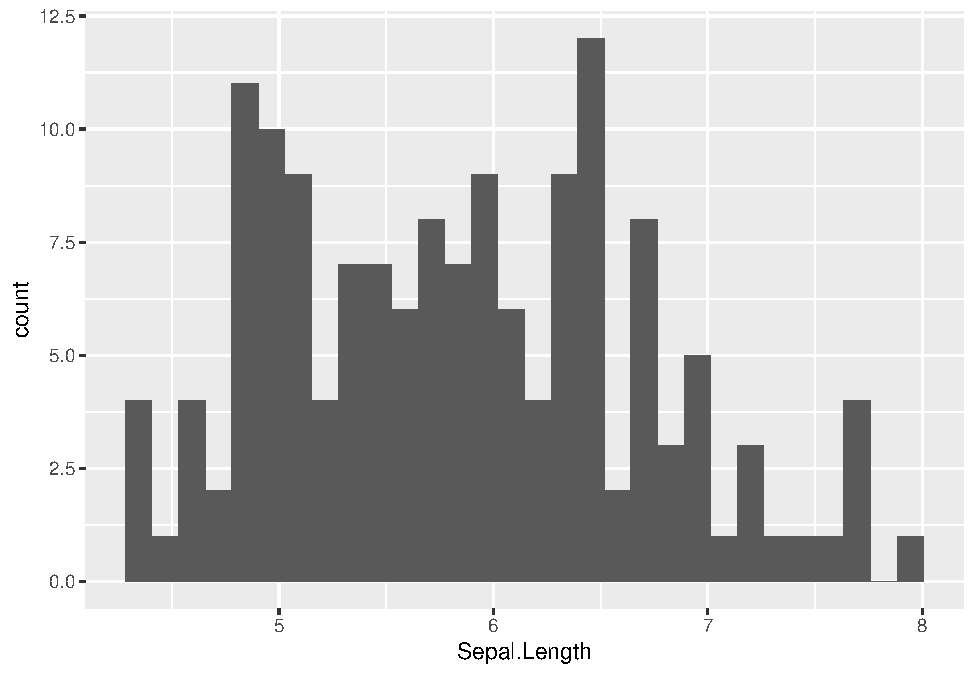
\includegraphics{CFH_R_bookdown_files/figure-latex/unnamed-chunk-6-1.pdf}

Pakete müssen zu Beginn jeder R Session neu geladen werden. Deswegen schreiben wir in der Regel ganz an den Anfang unseres Skripts gleich mehrere Zeilen, mit \texttt{library()} Befehlen für alle R Pakete, die wir für unsere Analyse benötigen werden.

In R gibt es eine Möglichkeit, ein Paket vorübergehend zu laden, ohne die Funktion \texttt{library()} zu verwenden. Um dies zu tun, können Sie einfach die Notation \texttt{package::funktion} verwenden. Diese Notation sagt R einfach, dass es das Paket nur für diesen einen Codeabschnitt laden soll. Zum Beispiel könnte ich die Funktion \texttt{ggplot} aus dem Paket \texttt{ggplot2} wie folgt verwenden:

\begin{Shaded}
\begin{Highlighting}[]
\NormalTok{ggplot2}\SpecialCharTok{::}\FunctionTok{ggplot}\NormalTok{(}\AttributeTok{data =}\NormalTok{ iris, }\FunctionTok{aes}\NormalTok{(}\AttributeTok{x =}\NormalTok{ Sepal.Length)) }\SpecialCharTok{+} 
  \FunctionTok{geom\_histogram}\NormalTok{()}
\end{Highlighting}
\end{Shaded}

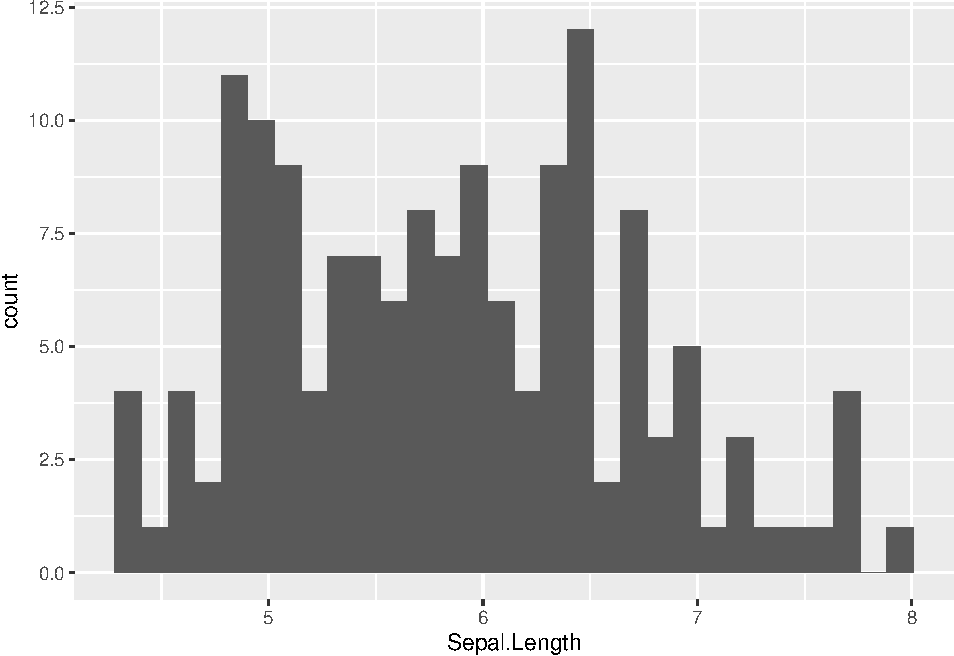
\includegraphics{CFH_R_bookdown_files/figure-latex/unnamed-chunk-7-1.pdf}

Ein Vorteil der Notation ``package::function'' ist, dass für jeden, der den Code liest, sofort klar ist, welches Paket die Funktion enthält. Ein Nachteil ist jedoch, dass Sie, wenn Sie eine Funktion aus einem Paket häufig verwenden, gezwungen sind, den Paketnamen ständig neu einzugeben. Sie können jede Methode verwenden, die für Sie sinnvoll ist.

\hypertarget{datenformate}{%
\chapter{Datenformate}\label{datenformate}}

\begin{figure}
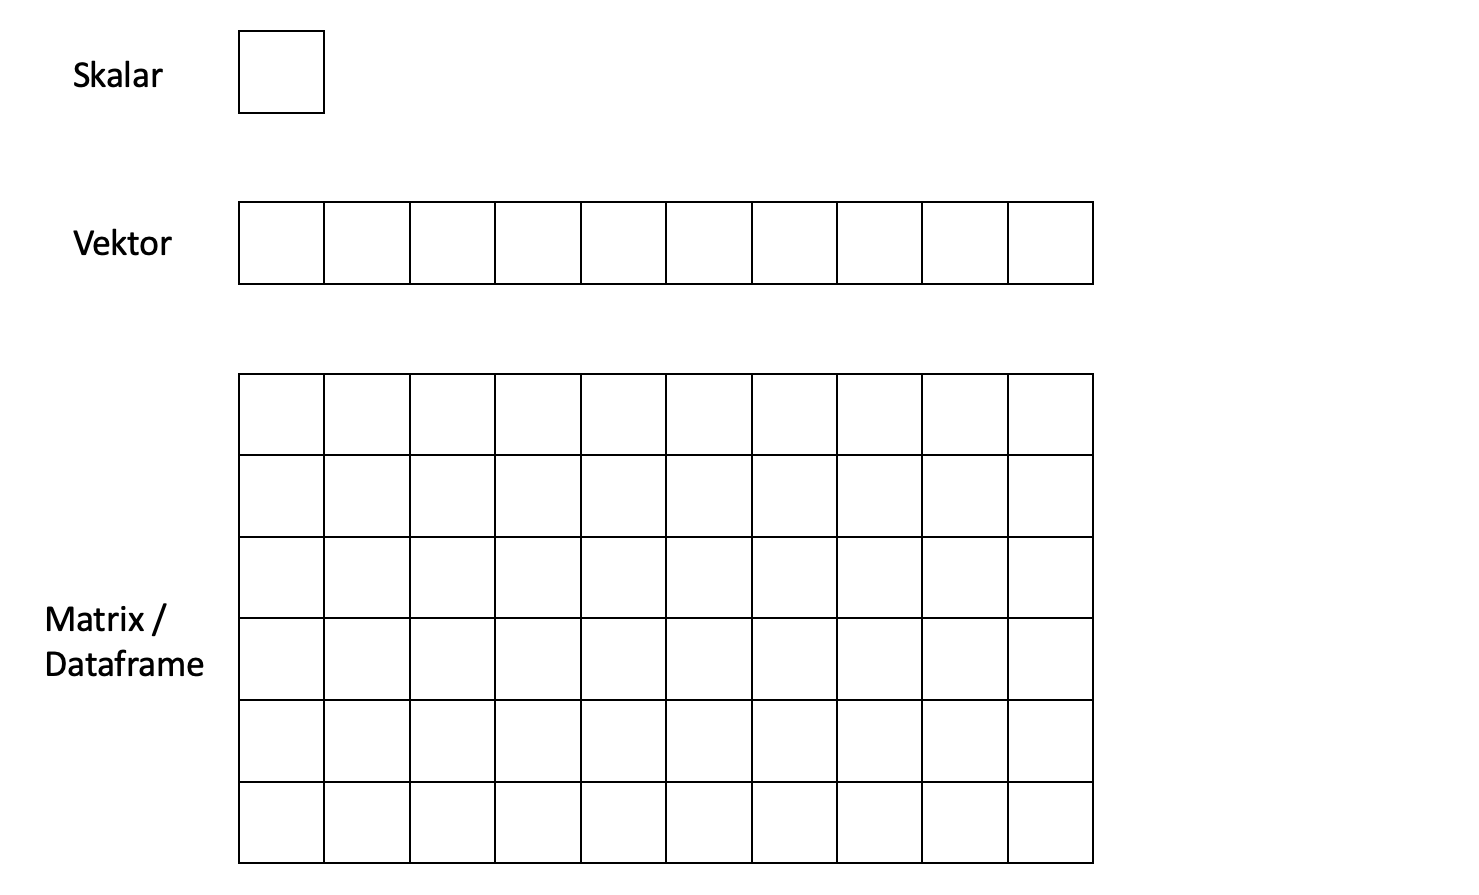
\includegraphics[width=20.54in]{images/Datenformat_1} \caption{Skalar, Vektor, Matrix}\label{fig:unnamed-chunk-8}
\end{figure}

\hypertarget{skalar}{%
\section{Skalar}\label{skalar}}

Der einfachste Objekttyp in R ist der \textbf{Skalar}. Ein Skalar Objekt ist einfach nur ein einzelner Wert, z.B. eine Zahl oder ein Wort.

Hier sind einige Beispiele für numerische Skalar Objekte:

\begin{Shaded}
\begin{Highlighting}[]
\CommentTok{\# Examples of numeric scalars}
\NormalTok{a }\OtherTok{\textless{}{-}} \DecValTok{100}
\NormalTok{b }\OtherTok{\textless{}{-}} \DecValTok{3} \SpecialCharTok{/} \DecValTok{100}
\NormalTok{c }\OtherTok{\textless{}{-}}\NormalTok{ (a }\SpecialCharTok{+}\NormalTok{ b) }\SpecialCharTok{/}\NormalTok{ b}
\end{Highlighting}
\end{Shaded}

Skalare müssen nicht numerisch sein, sondern auch Worte. Wortobjekte heißen in R \textbf{characters} (aka strings). In R schreibt man characters immer in Anführungszeichen \texttt{""}. Hier sind einige Beispiele für character Skalare:

\begin{Shaded}
\begin{Highlighting}[]
\CommentTok{\# Beispiele für character Skalare}
\NormalTok{d }\OtherTok{\textless{}{-}} \StringTok{"Psychologe"}
\NormalTok{e }\OtherTok{\textless{}{-}} \StringTok{"Zigarre"}
\NormalTok{f }\OtherTok{\textless{}{-}} \StringTok{"Haben Psychologen wirklich alle Bärte und rauchen Zigarre?"}
\end{Highlighting}
\end{Shaded}

Wie Sie sich vermutlich vorstellen können, behandelt R numerische und character Skalare unterschiedlich. Zum Beispiel lassen sich mir numerischen Skalaren grundlegende arithmetische Operationen durchfühlen (Addition, Subtraktion, Multiplikation\ldots) -- das funktioniert mit character Skalaren nicht.
Wenn Sie dennoch probieren numerische Operationen auf character Skalare anzuwenden, bekommen Sie eine Fehlermeldung, so wie diese:

\begin{Shaded}
\begin{Highlighting}[]
\NormalTok{a }\OtherTok{=} \StringTok{"1"}
\NormalTok{b }\OtherTok{=} \StringTok{"2"}
\NormalTok{a }\SpecialCharTok{+}\NormalTok{ b}
\end{Highlighting}
\end{Shaded}

\emph{``Fehler in a + b : nicht-numerisches Argument für binären Operator''}

\hypertarget{vektor}{%
\section{Vektor}\label{vektor}}

Machen wir weiter mit \texttt{Vektoren}. Ein Vektor Objekt ist einfach eine Kombination mehrerer Skalare in einem einzelnen Objekt (z.B. eine Zahlen- oder Wortreihe).
Zum Beispiel könnten die Zahlen von 1-10 in einen Vektor mit der Länge 10 kombiniert werden. Oder die Buchstaben des Alphabets könnten in einen Vektor mit der Länge 26 gespeichert werden. Genau wie Skalare, können Vektoren numerisch oder characters sein (Aber nicht beides auf einmal!)

Die einfachste Art einen Vektor zu erstellen ist mit der \texttt{c()} Funktion. Das c steht für ``concatenate'', was auf Englisch so viel heißt wie ``zusammenbringen''. Die \texttt{c()} Funktion nimmt mehrere Skalare als Input und erstellt einen Vektor, der diese Objekte enthält.

Wenn man\texttt{c()} benutzt, muss man immer ein \textbf{Komma} zwischen die Objekte setzen (Skalare oder Vektoren), die man kombinieren möchte.

Lassen Sie uns die \texttt{c()} Funktion nutzen um einen Vektor zu erstellen der \texttt{a} heißt und die Zahlen von 1 bis 7 enthält

Let's use the \texttt{c()} function to create a vector called \texttt{a} containing the integers from 1 to 5.

\begin{Shaded}
\begin{Highlighting}[]
\NormalTok{a }\OtherTok{=} \FunctionTok{c}\NormalTok{(}\DecValTok{1}\NormalTok{, }\DecValTok{2}\NormalTok{, }\DecValTok{3}\NormalTok{, }\DecValTok{4}\NormalTok{, }\DecValTok{5}\NormalTok{, }\DecValTok{6}\NormalTok{, }\DecValTok{7}\NormalTok{)}
\CommentTok{\# Das Ergebnis ausgeben}
\NormalTok{a}
\end{Highlighting}
\end{Shaded}

\begin{verbatim}
## [1] 1 2 3 4 5 6 7
\end{verbatim}

Sie können auch character Vektoren erstellen, indem Sie die \texttt{c()} auf einzelne character Skalare Funktion anwenden:

\begin{Shaded}
\begin{Highlighting}[]
\NormalTok{char.vec }\OtherTok{=} \FunctionTok{c}\NormalTok{(}\StringTok{"Freud"}\NormalTok{, }\StringTok{"Wundt"}\NormalTok{, }\StringTok{"Bandura"}\NormalTok{, }\StringTok{"Watson"}\NormalTok{, }\StringTok{"Jung"}\NormalTok{)}
\CommentTok{\# Das Ergebnis ausgeben}
\NormalTok{char.vec}
\end{Highlighting}
\end{Shaded}

\begin{verbatim}
## [1] "Freud"   "Wundt"   "Bandura" "Watson"  "Jung"
\end{verbatim}

\hypertarget{vektor-typen}{%
\subsection{Vektor Typen}\label{vektor-typen}}

Vektoren sind ein zentrales Element von R. Ein Vektor kann Zahlen, Buchstaben oder logische Werte enthalten, aber niemals eine Kombination

Der Vektor ist die Entsprechung der \textbf{Variable} und die Skalare, aus denen der Vektor besteht sind die \textbf{Merkmalsausprägungen} der Variable.

\hypertarget{faktor-variablen}{%
\subsection{Faktor Variablen}\label{faktor-variablen}}

Wir haben bereits gelernt, wie man einen Vektor aus character Objekten erstellt. Manchmal brauchen wir in R jedoch Variablen, die nicht nur Worte enthalten, sondern dem Programm mitteilen, dass es sich um feste Gruppen oder \textbf{Kategorien} handelt. Es geht also nicht nur um eine ``Sammlung'' von Worten (z.B. Nachnamen von Probanden), sondern um festgelegte Analyseeinheiten. Solche Variablen heißen in R \texttt{factor}.

In einer factor Variable ist jeder Kategorie eine Zahl zugeordnet (z.B. 1 = männlich, 2 = weiblich).

Um Faktor Variablen zu erstellen, machen wie einen Vorgang, den man \textbf{Kodieren} nennt und das geht so:

Wir haben einen Vektor mit Codes 1 und 2 für männlich und weiblich vorliegen:

\begin{Shaded}
\begin{Highlighting}[]
\NormalTok{geschlecht }\OtherTok{=} \FunctionTok{c}\NormalTok{(}\DecValTok{1}\NormalTok{, }\DecValTok{2}\NormalTok{, }\DecValTok{2}\NormalTok{, }\DecValTok{1}\NormalTok{, }\DecValTok{2}\NormalTok{)}
\CommentTok{\# Das Ergebnis ausgeben}
\NormalTok{geschlecht}
\end{Highlighting}
\end{Shaded}

\begin{verbatim}
## [1] 1 2 2 1 2
\end{verbatim}

In dieser Form erkennt R diesen Vektor als numerische Variable. Um Sie in einen Faktor umzuwandeln, definieren wir die Zahlen (1 und 2) als \texttt{levels} des Faktors und geben dann jedem level einen Namen (\texttt{labels}):

\begin{Shaded}
\begin{Highlighting}[]
\NormalTok{geschlecht }\OtherTok{=} \FunctionTok{factor}\NormalTok{(geschlecht, }\AttributeTok{levels =} \FunctionTok{c}\NormalTok{(}\DecValTok{1}\NormalTok{,}\DecValTok{2}\NormalTok{), }\AttributeTok{labels =} \FunctionTok{c}\NormalTok{(}\StringTok{"männlich"}\NormalTok{, }\StringTok{"weiblich"}\NormalTok{))}
\CommentTok{\# Das Ergebnis ausgeben}
\NormalTok{geschlecht}
\end{Highlighting}
\end{Shaded}

\begin{verbatim}
## [1] männlich weiblich weiblich männlich weiblich
## Levels: männlich weiblich
\end{verbatim}

Das Ergebnis ist eine codierte Faktorvariable. Wenn wir Sie uns ausgeben lassen erhalten wir unter den Merkmalsausprägungen eine Liste mit den einzelnen Kategorien (levels) des Faktors.

R wird uns für Faktoren alle Ergebnisse nach der \textbf{Reihenfolge} der levels anzeigen. Wenn wir keine Faktorvariable haben, sondern eine character Variable funktioniert die Reihenfolge immer alphabetisch.

\hypertarget{vektor-indizierung}{%
\subsection{Vektor Indizierung}\label{vektor-indizierung}}

Manchmal möchten wir wieder einen einzelnen Skalar auswählen, der als Teil von einem Vektor gespeichert ist. Diese \textbf{Auswahl} eines Einzelelements nennt man \textbf{Indizierung}. Die Auswahl eines kleineren Objekts aus einem größeren Objekt funktioniert in R immer mit \texttt{{[}{]}}.

Benötigen wir aus einem Vektor z.B. genau den 3. Skalar, schreiben wir einfach eine 3 in eckige Klammern hinter den Vektor.

\begin{Shaded}
\begin{Highlighting}[]
\NormalTok{char.vec }\OtherTok{=} \FunctionTok{c}\NormalTok{(}\StringTok{"Freud"}\NormalTok{, }\StringTok{"Wundt"}\NormalTok{, }\StringTok{"Bandura"}\NormalTok{, }\StringTok{"Watson"}\NormalTok{, }\StringTok{"Jung"}\NormalTok{)}
\CommentTok{\# Das Ergebnis ausgeben}
\NormalTok{char.vec[}\DecValTok{5}\NormalTok{]}
\end{Highlighting}
\end{Shaded}

\begin{verbatim}
## [1] "Jung"
\end{verbatim}

\hypertarget{matrizen-und-dataframes}{%
\section{Matrizen und Dataframes}\label{matrizen-und-dataframes}}

In der Psychologie beobachten wir für unsere Studien fast immer mehr als eine Variable. Wir könnten diese alle in einzelnen Vektoren speichern und uns die Objektnamen merken. Z.B.

\begin{Shaded}
\begin{Highlighting}[]
\NormalTok{Name }\OtherTok{=} \FunctionTok{c}\NormalTok{(}\StringTok{"Max"}\NormalTok{, }\StringTok{"Maja"}\NormalTok{, }\StringTok{"Mia"}\NormalTok{, }\StringTok{"Moritz"}\NormalTok{, }\StringTok{"Markus"}\NormalTok{)}
\NormalTok{Alter }\OtherTok{=} \FunctionTok{c}\NormalTok{(}\DecValTok{20}\NormalTok{, }\DecValTok{31}\NormalTok{, }\DecValTok{25}\NormalTok{, }\DecValTok{34}\NormalTok{, }\DecValTok{51}\NormalTok{)}
\NormalTok{Diagnose }\OtherTok{=} \FunctionTok{c}\NormalTok{(}\StringTok{"Depression"}\NormalTok{, }\StringTok{"Zwangsstörung"}\NormalTok{, }\StringTok{"Depression"}\NormalTok{, }\StringTok{"Soziale Phobie"}\NormalTok{, }\StringTok{"Depression"}\NormalTok{)}
\end{Highlighting}
\end{Shaded}

\hypertarget{erstellen-von-datenmatrizen}{%
\subsection{Erstellen von Datenmatrizen}\label{erstellen-von-datenmatrizen}}

Praktischer ist es, die einzelnen Vektoren in Tabellenform zu speichern, der \textbf{Datenmatrix}. In R heißen Datenmatrizen \texttt{data.frame}. Wir können die Vektoren folgendermaßen zu einem data.frame kombinieren:

\begin{Shaded}
\begin{Highlighting}[]
\NormalTok{df }\OtherTok{=} \FunctionTok{data.frame}\NormalTok{(Name, Alter, Diagnose)}
\CommentTok{\# Das Ergebnis ausgeben}
\NormalTok{df}
\end{Highlighting}
\end{Shaded}

\begin{verbatim}
##     Name Alter       Diagnose
## 1    Max    20     Depression
## 2   Maja    31  Zwangsstörung
## 3    Mia    25     Depression
## 4 Moritz    34 Soziale Phobie
## 5 Markus    51     Depression
\end{verbatim}

Wie in jeder Datenmatrix entsprechen die \textbf{Zeilen} den einzelnen Personen (Fällen) und die \textbf{Spalten} den Variablen.

R bezeichnet Zeilen und Spalten als \textbf{rows} und \textbf{columns}. Wollen wir z.B. wissen, wie viele Zeilen der data.frame hat, können wir \texttt{nrow()} benutzen. Für die Anzahl der Spalten nehmen wir \texttt{ncol()}:

\begin{Shaded}
\begin{Highlighting}[]
\FunctionTok{nrow}\NormalTok{(df)}
\end{Highlighting}
\end{Shaded}

\begin{verbatim}
## [1] 5
\end{verbatim}

\begin{Shaded}
\begin{Highlighting}[]
\FunctionTok{ncol}\NormalTok{(df)}
\end{Highlighting}
\end{Shaded}

\begin{verbatim}
## [1] 3
\end{verbatim}

Wenn wir die einzelnen Vektoren nicht bereits vorher definiert haben, können wir auch alles in einem Schritt machen. Das Ergebnis ist das gleiche:

\begin{Shaded}
\begin{Highlighting}[]
\NormalTok{df }\OtherTok{=} \FunctionTok{data.frame}\NormalTok{(}\StringTok{"Name"} \OtherTok{=} \FunctionTok{c}\NormalTok{(}\StringTok{"Max"}\NormalTok{, }\StringTok{"Maja"}\NormalTok{, }\StringTok{"Mia"}\NormalTok{, }\StringTok{"Moritz"}\NormalTok{, }\StringTok{"Markus"}\NormalTok{),}
                \StringTok{"Alter"} \OtherTok{=} \FunctionTok{c}\NormalTok{(}\DecValTok{20}\NormalTok{, }\DecValTok{31}\NormalTok{, }\DecValTok{25}\NormalTok{, }\DecValTok{34}\NormalTok{, }\DecValTok{51}\NormalTok{),}
                \StringTok{"Diagnose"} \OtherTok{=} \FunctionTok{c}\NormalTok{(}\StringTok{"Depression"}\NormalTok{, }\StringTok{"Zwangsstörung"}\NormalTok{, }\StringTok{"Depression"}\NormalTok{, }\StringTok{"Soziale Phobie"}\NormalTok{, }\StringTok{"Depression"}\NormalTok{)}
\NormalTok{                )}
\CommentTok{\# Das Ergebnis ausgeben}
\NormalTok{df}
\end{Highlighting}
\end{Shaded}

\begin{verbatim}
##     Name Alter       Diagnose
## 1    Max    20     Depression
## 2   Maja    31  Zwangsstörung
## 3    Mia    25     Depression
## 4 Moritz    34 Soziale Phobie
## 5 Markus    51     Depression
\end{verbatim}

Wollen wir wieder eine einzelne Variable aus dem benutzen, können wir diese über das \texttt{\$} Zeichen anwählen:

\begin{Shaded}
\begin{Highlighting}[]
\NormalTok{df}\SpecialCharTok{$}\NormalTok{Alter}
\end{Highlighting}
\end{Shaded}

\begin{verbatim}
## [1] 20 31 25 34 51
\end{verbatim}

\hypertarget{indizierung}{%
\subsection{Indizierung}\label{indizierung}}

Wollen wir aus dem data.frame wieder einzelne Elemente benutzen, nutzen wir wieder die Indizierung. Auch hier brauchen wir die \texttt{{[}{]}}. Da wir im data.frame Zeilen und Spalten haben, brauchen wir eine Möglichkeit beides auszuwählen, wie ein Curser der von links nach rechts, bzw. von oben nach unten läuft.

Wir trennen dafür unsere \texttt{{[}{]}} mit einem Komma \texttt{{[},{]}}. Alles was \textbf{links vom Komma} steht bezieht sich auf Zeilen alles \textbf{rechts vom Komma} bezieht sich auf Spalten.

Lassen Sie uns einmal die Zelle in der 1. Zeile (also die 1. Person) und der 3. Variable auswählen:

\begin{Shaded}
\begin{Highlighting}[]
\NormalTok{df[}\DecValTok{1}\NormalTok{,}\DecValTok{3}\NormalTok{]}
\end{Highlighting}
\end{Shaded}

\begin{verbatim}
## [1] Depression
## Levels: Depression Soziale Phobie Zwangsstörung
\end{verbatim}

Lassen wir die Zahl vor dem Komma weg, bekommen wir alle Werte aus der Spalte:

\begin{Shaded}
\begin{Highlighting}[]
\NormalTok{df[,}\DecValTok{3}\NormalTok{]}
\end{Highlighting}
\end{Shaded}

\begin{verbatim}
## [1] Depression     Zwangsstörung  Depression     Soziale Phobie Depression    
## Levels: Depression Soziale Phobie Zwangsstörung
\end{verbatim}

Lassen wir die Zahl nach dem Komma weg, bekommen wir alle Werte aus der Reihe:

\begin{Shaded}
\begin{Highlighting}[]
\NormalTok{df[}\DecValTok{1}\NormalTok{,]}
\end{Highlighting}
\end{Shaded}

\begin{verbatim}
##   Name Alter   Diagnose
## 1  Max    20 Depression
\end{verbatim}

\hypertarget{daten-erstellen}{%
\chapter{Daten erstellen}\label{daten-erstellen}}

\hypertarget{manuell}{%
\section{Manuell}\label{manuell}}

Die manuelle Eingabe von Daten erfolgt über die \texttt{c()} Funktion. Mit ihrer Hilfe können wir Skalare zu Vektoren verbinden\ldots{}

\begin{Shaded}
\begin{Highlighting}[]
\NormalTok{a }\OtherTok{=} \FunctionTok{c}\NormalTok{(}\DecValTok{1}\NormalTok{, }\DecValTok{2}\NormalTok{, }\DecValTok{4}\NormalTok{, }\DecValTok{6}\NormalTok{, }\DecValTok{1}\NormalTok{)}
\end{Highlighting}
\end{Shaded}

\ldots mehrere Vektoren aneinanderhängen\ldots{}

\begin{Shaded}
\begin{Highlighting}[]
\NormalTok{a }\OtherTok{=} \FunctionTok{c}\NormalTok{(}\DecValTok{1}\NormalTok{, }\DecValTok{2}\NormalTok{, }\DecValTok{4}\NormalTok{, }\DecValTok{6}\NormalTok{, }\DecValTok{1}\NormalTok{)}
\NormalTok{b }\OtherTok{=} \FunctionTok{c}\NormalTok{(}\DecValTok{2}\NormalTok{, }\DecValTok{3}\NormalTok{)}
\NormalTok{c }\OtherTok{=} \FunctionTok{c}\NormalTok{(a, b)}
\NormalTok{c}
\end{Highlighting}
\end{Shaded}

\begin{verbatim}
## [1] 1 2 4 6 1 2 3
\end{verbatim}

\ldots und Vektoren gleicher Länge zu data.frames kombinieren:

\begin{Shaded}
\begin{Highlighting}[]
\NormalTok{daten }\OtherTok{=} \FunctionTok{data.frame}\NormalTok{(}\AttributeTok{aufmerksamkeit =} \FunctionTok{c}\NormalTok{(}\DecValTok{58}\NormalTok{, }\DecValTok{46}\NormalTok{, }\DecValTok{29}\NormalTok{, }\DecValTok{51}\NormalTok{),}
                   \AttributeTok{gedaechtnis =} \FunctionTok{c}\NormalTok{(}\DecValTok{22}\NormalTok{, }\DecValTok{67}\NormalTok{, }\DecValTok{22}\NormalTok{, }\DecValTok{31}\NormalTok{))}
\NormalTok{daten}
\end{Highlighting}
\end{Shaded}

\begin{verbatim}
##   aufmerksamkeit gedaechtnis
## 1             58          22
## 2             46          67
## 3             29          22
## 4             51          31
\end{verbatim}

\hypertarget{automatisch}{%
\section{Automatisch}\label{automatisch}}

Wir haben bereits die \texttt{c()} Funktion gelernt.

Die \texttt{c()} Funktion ist die einfachste Art einen Vektor zu erstellen, sie ist aber vermutlich auch die umständlichste. Stellen Sie sich zum Beispiel vor, Sie wollen einen Vektor erstellen, der alle Zahlen von 0 bis 100 enthält. Diese Zahlen wollen Sie definitiv nicht alle in die Klammer von \texttt{c()} eintippen.

Glücklicherweise hat R viele eingebaute Funktionen, um leicht automatisch numerische Vektoren zu erstellen.

Lassen Sie uns mit dreien davon starten\texttt{a:b}, \texttt{seq()}, and \texttt{rep()}:

\begin{longtable}[]{@{}
  >{\raggedright\arraybackslash}p{(\columnwidth - 4\tabcolsep) * \real{0.3881}}
  >{\raggedright\arraybackslash}p{(\columnwidth - 4\tabcolsep) * \real{0.4478}}
  >{\raggedright\arraybackslash}p{(\columnwidth - 4\tabcolsep) * \real{0.1642}}@{}}
\toprule()
\begin{minipage}[b]{\linewidth}\raggedright
Funktion
\end{minipage} & \begin{minipage}[b]{\linewidth}\raggedright
Beispiel
\end{minipage} & \begin{minipage}[b]{\linewidth}\raggedright
Ergebnis
\end{minipage} \\
\midrule()
\endhead
\texttt{c(a,\ b,\ ...)} & \texttt{c(1,\ 5,\ 9)} & 1, 5, 9 \\
\texttt{a:b} & \texttt{1:5} & 1, 2, 3, 4, 5 \\
\texttt{seq(from,\ to,\ by,\ length.out)} & \texttt{seq(from\ =\ 0,\ to\ =\ 6,\ by\ =\ 2)} & 0, 2, 4, 6 \\
\texttt{rep(x,\ times,\ each,\ length.out)} & \texttt{rep(c(7,\ 8),\ times\ =\ 2,\ each\ =\ 2)} & 7, 7, 8, 8, 7, 7, 8, 8 \\
\bottomrule()
\end{longtable}

\hypertarget{zufuxe4llig}{%
\section{Zufällig}\label{zufuxe4llig}}

In R haben Sie die möglichkeit Daten anhand einer Wahrscheinlichkeitsverteilung zu simulieren.

Wollen wir beispielsweise eine normalverteilte Variable mit zufälligen Werten erstellen, können wir die \texttt{rnorm()} Funktion nutzen. Dafür müssen wir lediglich angeben, wie viele Werte wir haben wollen (\texttt{n}) und welchen Mittelwert (\texttt{mean}) und welche Standardabweichung (\texttt{sd}) die Verteilung haben soll:

\begin{Shaded}
\begin{Highlighting}[]
\FunctionTok{rnorm}\NormalTok{(}\AttributeTok{n =} \DecValTok{20}\NormalTok{, }\AttributeTok{mean =} \DecValTok{0}\NormalTok{, }\AttributeTok{sd =} \DecValTok{1}\NormalTok{)}
\end{Highlighting}
\end{Shaded}

\begin{verbatim}
##  [1]  0.27937464 -0.64817022 -1.21771039 -0.53721254  1.55755864  0.42285519
##  [7] -1.42577481  2.29665855  0.53761077 -0.09185485  1.23517906  0.63837105
## [13] -0.53382421 -0.86115246  0.52379564  0.11576233  1.21410540 -0.53969760
## [19] -1.53772456  0.55406633
\end{verbatim}

\hypertarget{daten-importieren-und-speichern}{%
\chapter{Daten importieren und speichern}\label{daten-importieren-und-speichern}}

In diesem Kapitel werden wir die Grundlagen der R-Objektverwaltung behandeln. Es wird erläutert, wie Sie neue Objekte, z. B. externe Datensätze, in R laden, wie Sie die bereits vorhandenen Objekte verwalten und wie Sie Objekte aus R in externe Dateien exportieren, die Sie mit anderen Personen teilen oder für Ihre eigene zukünftige Verwendung speichern können.

\hypertarget{funktionen-zur-organisation-des-workspace}{%
\section{Funktionen zur Organisation des Workspace}\label{funktionen-zur-organisation-des-workspace}}

In diesem Kapitel werden wir einige hilfreiche Funktionen zur Verwaltung Ihres Arbeitsbereichs vorstellen:

\begin{longtable}[]{@{}
  >{\raggedright\arraybackslash}p{(\columnwidth - 2\tabcolsep) * \real{0.4167}}
  >{\raggedright\arraybackslash}p{(\columnwidth - 2\tabcolsep) * \real{0.5833}}@{}}
\toprule()
\begin{minipage}[b]{\linewidth}\raggedright
Code
\end{minipage} & \begin{minipage}[b]{\linewidth}\raggedright
Description
\end{minipage} \\
\midrule()
\endhead
\texttt{ls()} & Alle Objekte im aktuellen Arbeitsbereich anzeigen \\
\texttt{rm(x,\ y,\ ..)} & Entfernt die Objete \texttt{y}, \texttt{y}\ldots{} aus dem Arbeitsbereich \\
\texttt{rm(list\ =\ ls())} & Entfernt \emph{alle} Objekte aus dem Arbeitsbereich \\
\texttt{getwd()} & Zeigt das aktuelle Arbeitsverzeichnis an \\
\texttt{setwd(file\ =\ "dir)} & Wechselt das Arbeitsverzeichnis zu einem bestimmten Dateipfad \\
\texttt{list.files()} & Zeigt die Namen aller Dateien im Arbeitsverzeichnis an \\
\texttt{write.table(x,\ file\ =\ "mydata.txt",\ sep)} & writes the object \texttt{x} to a text file called \texttt{mydata.txt}. Define how the columns will be separated with \texttt{sep} (e.g.; \texttt{sep\ =\ ","} for a comma--separated file, and \texttt{sep\ =\ \textbackslash{}t"} for a tab--separated file). \\
\texttt{write\_rds(x,"meineDaten.rds)} & Speichert Objekt x in das R Objekt \texttt{meineDaten.rds} \\
\texttt{save.image(file\ =\ "meineSession.RData")} & Speichert \emph{alle} Objekte aus dem Arbeitsbereich nach \texttt{meineSession.RData} \\
\texttt{read\_rds}(``Daten.rds'')\texttt{\textbar{}Läd\ das\ rds\ Objekt}Daten.rds\texttt{\textbar{}\ \textbar{}}read.csv\texttt{("Daten.csv")} & Läd den csv Datensatz \texttt{Daten.csv} \\
\texttt{foreign::read.spss("Daten.sav")} & Läd den SPSS Datensatz \texttt{Daten.sav} \\
\texttt{read.csv("Daten.csv")} & Läd den csv Datensatz \texttt{Daten.csv} \\
\texttt{readxl::read\_xlsx("Daten.xlsx")} & Läd den Excel Datensatz \texttt{Daten.xlsx} \\
\bottomrule()
\end{longtable}

Ihr Computer ist ein Labyrinth aus Ordnern und Dateien. Wenn Sie außerhalb von R eine bestimmte Datei öffnen möchten, öffnen Sie wahrscheinlich ein Explorer-Fenster, mit dem Sie die Ordner auf Ihrem Computer visuell durchsuchen können. Oder Sie wählen die zuletzt geöffneten Dateien aus oder geben den Namen der Datei in ein Suchfeld ein, um den Computer die Suche für Sie übernehmen zu lassen. Während dieses Vorgehen normalerweise für nicht-programmierende Aufgaben funktioniert, ist es für R ein No-Go. Das Hauptproblem ist, dass Sie bei all diesen Methoden Ihre Ordner visuell durchsuchen und die Maus bewegen müssen, um Ordner und Dateien auszuwählen, die dem Gesuchten entsprechen. Wenn Sie in R programmieren, müssen Sie alle Schritte in Ihren Analysen so spezifizieren, dass sie von anderen und von Ihnen selbst leicht nachvollzogen werden können. Das bedeutet, dass Sie nicht einfach sagen können: ``Finde diese eine Datei, die ich mir vor einer Woche gemailt habe'' oder ``Suche nach einer Datei, die so aussieht wie''MeinFoto.jpg''. Stattdessen müssen Sie in der Lage sein, R-Code zu schreiben, der R genau sagt, wo wichtige Dateien zu finden sind - entweder auf Ihrem Computer oder im Internet.

Um diese Aufgabe zu erleichtern, verwendet R Arbeitsverzeichnisse.

\hypertarget{arbeitsverzeichnis-working-directory}{%
\section{Arbeitsverzeichnis (Working Directory)}\label{arbeitsverzeichnis-working-directory}}

Das Arbeitsverzeichnis ist lediglich ein Dateipfad auf Ihrem Computer, der den Standardspeicherort aller Dateien festlegt, die Sie in R einlesen oder aus R heraus speichern. Mit anderen Worten, ein Arbeitsverzeichnis ist wie eine kleine Kiste irgendwo auf Ihrem Computer, die an ein bestimmtes Analyseprojekt gebunden ist. Wenn Sie R auffordern, einen Datensatz zu importieren wird davon ausgegangen, dass sich die Datei in Ihrem Arbeitsverzeichnis befindet.

Sie können zu jedem Zeitpunkt nur ein Arbeitsverzeichnis aktiv haben. Das aktive Arbeitsverzeichnis wird als Ihr aktuelles Arbeitsverzeichnis bezeichnet.

\hypertarget{working-environment}{%
\section{Working Environment}\label{working-environment}}

Der Arbeitsbereich (auch als Arbeitsumgebung bezeichnet) enthält alle Objekte und Funktionen, die Sie entweder in der aktuellen Sitzung definiert oder aus einer früheren Sitzung geladen haben. Als Sie RStudio zum ersten Mal starteten, war die Arbeitsumgebung leer, da Sie keine neuen Objekte oder Funktionen erstellt hatten. Wenn Sie jedoch neue Objekte und Funktionen mit dem Zuweisungsoperator = definiert haben, wurden diese neuen Objekte in Ihrer Arbeitsumgebung gespeichert. Wenn Sie RStudio nach der Definition neuer Objekte schlossen, erhielten Sie wahrscheinlich eine Meldung mit der Frage ``Save workspace image\ldots?''. Damit möchte RStudio Sie fragen, ob Sie alle derzeit in Ihrem Arbeitsbereich definierten Objekte als Bilddatei auf Ihrem Computer speichern möchten.

\begin{Shaded}
\begin{Highlighting}[]
\CommentTok{\# getwd()}
\end{Highlighting}
\end{Shaded}

\hypertarget{daten-importieren}{%
\section{Daten importieren}\label{daten-importieren}}

Wenn Sie Daten in Ihrem Arbeitsverzeichnis haben, können Sie diese nun in R einlesen und dort mit ihnen rechnen. Nehmen wir an, Sie haben in Ihrem Arbeitsverzeichnis einen Ordner mit dem Namen \texttt{data}.

Je nachdem in welchem Format die Daten vorliegen, muss ein eigener Befehl genutzt werden. Teilweise braucht man hier auch eigene Pakete (z.B. Excel- oder SPSS-Format).

\hypertarget{rds-format}{%
\subsection{rds-Format}\label{rds-format}}

.rds ist das R-eigene Format. Es speichert alle Objekte die es in R gibt, also potentiell nicht nur Datensätze, sondern auch Testergebnisse, Bilder, o.ä. mittels der Funktion \texttt{read\_rds()} können wir die Objekte einlesen. Dafür müssen wir das Paket \texttt{readr} installiert und mittels \texttt{library} eingelesen haben.

\begin{Shaded}
\begin{Highlighting}[]
\NormalTok{data }\OtherTok{=} \FunctionTok{load}\NormalTok{(}\AttributeTok{file =} \StringTok{"data/personality.RData"}\NormalTok{)}

\CommentTok{\# erste Zeilen des Datensatzes ansehen}
\FunctionTok{head}\NormalTok{(data)}
\end{Highlighting}
\end{Shaded}

\begin{verbatim}
## [1] "data"
\end{verbatim}

\hypertarget{csv-format}{%
\subsection{csv-Format}\label{csv-format}}

Das .csv Format (comma-separated-values) ist eines der gängigsten in der Statistik. Es lässt sich mit allen gebräuchlichen Tabellenprogrammen öffnen (also neben R auch mit Excel, Numbers, o.ä.).

Um einen .csv Datensatz einzulesen, speichern wir ihn mittel \texttt{read.csv()} in ein von uns benanntes Objekt. Dieses können wir nennen wie wir wollen, z.B. \texttt{data} (schön kurz):

\begin{Shaded}
\begin{Highlighting}[]
\NormalTok{data }\OtherTok{=} \FunctionTok{read.csv}\NormalTok{(}\StringTok{"data/personality.csv"}\NormalTok{)}

\CommentTok{\# erste Zeilen des Datensatzes ansehen}
\FunctionTok{head}\NormalTok{(data)}
\end{Highlighting}
\end{Shaded}

\begin{verbatim}
##   ID NEO_1_N NEO_2_E NEO_3_O NEO_4_V NEO_5_G NEO_6_N NEO_7_E NEO_8_O NEO_9_V
## 1  1       2       4       0       3       3       0       2       3       0
## 2  2       4       4       0       3       4       0       4       4       0
## 3  3       4       4       2       4       4       0       4       4       0
## 4  4       4       3       4       3       3       0       2       4       0
## 5  5       4       4       1       3       3       0       3       4       4
## 6  6       4       4       0       4       0       1       4       4       0
##   NEO_10_G NEO_11_N NEO_12_E NEO_13_O NEO_14_V NEO_15_G NEO_16_N NEO_17_E
## 1        3        4        1        2        0        4        4        3
## 2        4        1        0        3        0        3        4        4
## 3        4        4        2        4        0        0        4        4
## 4        3        0        0        2        0        0        4        4
## 5        3        1        4        4        0        0        4        4
## 6        2        0        0        4        0        0        4        4
##   NEO_18_O NEO_19_V NEO_20_G NEO_21_N NEO_22_E NEO_23_O NEO_24_V NEO_25_G
## 1        4        3        4        0        4        2        2        3
## 2        3        4        4        0        3        4        0        4
## 3        0        4        4        0        4        4        1        4
## 4        0        4        4        4        4        4        0        3
## 5        0        4        1        1        3        4        0        2
## 6        0        4        4        0        3        4        4        4
##   NEO_26_N NEO_27_E NEO_28_O NEO_29_V NEO_30_G NEO_31_N NEO_32_E NEO_33_O
## 1        4        4        4        2        4        3        0        0
## 2        2        0        1        0        4        4        4        4
## 3        4        0        0        0        1        4        4        3
## 4        0        0        0        0        0        4        4        0
## 5        0        4        4        2        4        4        3        4
## 6        0        0        4        2        0        4        3        2
##   NEO_34_V NEO_35_G NEO_36_N NEO_37_E NEO_38_O NEO_39_V NEO_40_G NEO_41_N
## 1        3        4        2        4        1        0        4        4
## 2        4        4        0        4        3        1        4        0
## 3        4        4        3        4        2        0        4        0
## 4        3        4        0        3        3        1        4        0
## 5        3        3        0        4        0        2        3        0
## 6        4        4        0        2        4        2        4        0
##   NEO_42_E NEO_43_O NEO_44_V NEO_45_G NEO_46_N NEO_47_E NEO_48_O NEO_49_V
## 1        2        1        4        0        4        4        3        3
## 2        2        4        0        2        4        0        4        4
## 3        4        4        4        0        4        0        4        4
## 4        2        2        0        0        4        4        3        3
## 5        0        2        0        1        4        0        2        3
## 6        0        4        0        0        4        0        2        4
##   NEO_50_G NEO_51_N NEO_52_E NEO_53_O NEO_54_V NEO_55_G NEO_56_N NEO_57_E
## 1        3        0        4        2        0        0        2        2
## 2        4        0        4        4        0        0        0        0
## 3        4        3        4        4        4        0        0        1
## 4        4        4        4        1        0        0        4        0
## 5        3        0        3        3        0        4        0        1
## 6        4        0        4        4        1        0        0        0
##   NEO_58_O NEO_59_V NEO_60_G
## 1        3        1        4
## 2        3        0        4
## 3        4        0        4
## 4        4        1        3
## 5        3        4        4
## 6        4        0        3
\end{verbatim}

\hypertarget{sav-format}{%
\subsection{sav-Format}\label{sav-format}}

Das .sav Format ist das Format in welchem SPSS Datensätze abgespeichert werden. Dies kommt gerade in den Sozialwissenschaften relativ häufig vor, weshalb wir diese Art von Datein auf jeden Fall einlesen können sollten.

Um einen .sav Datensatz einzulesen, speichern wir ihn mittel \texttt{read.spss()} in ein von uns benanntes Objekt. Dafür müssen wir das Paket \texttt{foreign} installiert und mittels \texttt{library} eingelesen haben. Damit R den Datensatz automatisch in einen data.frame speichert, geben wir als Zusatzoption \texttt{to.data.frame\ =\ TRUE} an:

\begin{Shaded}
\begin{Highlighting}[]
\FunctionTok{library}\NormalTok{(foreign)}
\NormalTok{data }\OtherTok{=} \FunctionTok{read.spss}\NormalTok{(}\StringTok{"data/personality.sav"}\NormalTok{, }\AttributeTok{to.data.frame =} \ConstantTok{TRUE}\NormalTok{)}

\CommentTok{\# erste Zeilen des Datensatzes ansehen}
\FunctionTok{head}\NormalTok{(data)}
\end{Highlighting}
\end{Shaded}

\begin{verbatim}
##   ID NEO_1_N NEO_2_E NEO_3_O NEO_4_V NEO_5_G NEO_6_N NEO_7_E NEO_8_O NEO_9_V
## 1  1       2       4       0       3       3       0       2       3       0
## 2  2       4       4       0       3       4       0       4       4       0
## 3  3       4       4       2       4       4       0       4       4       0
## 4  4       4       3       4       3       3       0       2       4       0
## 5  5       4       4       1       3       3       0       3       4       4
## 6  6       4       4       0       4       0       1       4       4       0
##   NEO_10_G NEO_11_N NEO_12_E NEO_13_O NEO_14_V NEO_15_G NEO_16_N NEO_17_E
## 1        3        4        1        2        0        4        4        3
## 2        4        1        0        3        0        3        4        4
## 3        4        4        2        4        0        0        4        4
## 4        3        0        0        2        0        0        4        4
## 5        3        1        4        4        0        0        4        4
## 6        2        0        0        4        0        0        4        4
##   NEO_18_O NEO_19_V NEO_20_G NEO_21_N NEO_22_E NEO_23_O NEO_24_V NEO_25_G
## 1        4        3        4        0        4        2        2        3
## 2        3        4        4        0        3        4        0        4
## 3        0        4        4        0        4        4        1        4
## 4        0        4        4        4        4        4        0        3
## 5        0        4        1        1        3        4        0        2
## 6        0        4        4        0        3        4        4        4
##   NEO_26_N NEO_27_E NEO_28_O NEO_29_V NEO_30_G NEO_31_N NEO_32_E NEO_33_O
## 1        4        4        4        2        4        3        0        0
## 2        2        0        1        0        4        4        4        4
## 3        4        0        0        0        1        4        4        3
## 4        0        0        0        0        0        4        4        0
## 5        0        4        4        2        4        4        3        4
## 6        0        0        4        2        0        4        3        2
##   NEO_34_V NEO_35_G NEO_36_N NEO_37_E NEO_38_O NEO_39_V NEO_40_G NEO_41_N
## 1        3        4        2        4        1        0        4        4
## 2        4        4        0        4        3        1        4        0
## 3        4        4        3        4        2        0        4        0
## 4        3        4        0        3        3        1        4        0
## 5        3        3        0        4        0        2        3        0
## 6        4        4        0        2        4        2        4        0
##   NEO_42_E NEO_43_O NEO_44_V NEO_45_G NEO_46_N NEO_47_E NEO_48_O NEO_49_V
## 1        2        1        4        0        4        4        3        3
## 2        2        4        0        2        4        0        4        4
## 3        4        4        4        0        4        0        4        4
## 4        2        2        0        0        4        4        3        3
## 5        0        2        0        1        4        0        2        3
## 6        0        4        0        0        4        0        2        4
##   NEO_50_G NEO_51_N NEO_52_E NEO_53_O NEO_54_V NEO_55_G NEO_56_N NEO_57_E
## 1        3        0        4        2        0        0        2        2
## 2        4        0        4        4        0        0        0        0
## 3        4        3        4        4        4        0        0        1
## 4        4        4        4        1        0        0        4        0
## 5        3        0        3        3        0        4        0        1
## 6        4        0        4        4        1        0        0        0
##   NEO_58_O NEO_59_V NEO_60_G
## 1        3        1        4
## 2        3        0        4
## 3        4        0        4
## 4        4        1        3
## 5        3        4        4
## 6        4        0        3
\end{verbatim}

\hypertarget{xlsx-format}{%
\subsection{xlsx-Format}\label{xlsx-format}}

Das .xlsx Format ist das Format in welchem Excel Datensätze abgespeichert werden. Auch das kommt oft vor, da es viele Forscher:innen vorziehen Daten in Excel Tabellen einzutragen.

Um einen .xlsx Datensatz einzulesen, speichern wir ihn mittel \texttt{read\_xlsx()} in ein von uns benanntes Objekt. Dafür müssen wir das Paket \texttt{readxl} installiert und mittels \texttt{library} eingelesen haben. Da in Excel Tabellen manchmal mehrere Arbeitsblätter (engl. ``sheets'') vorliegen, geben wir den Namen des Arbeitsblatt, welches wir brauchen, zusätzlich an:

\begin{Shaded}
\begin{Highlighting}[]
\FunctionTok{library}\NormalTok{(readxl)}
\NormalTok{data }\OtherTok{=} \FunctionTok{read\_xlsx}\NormalTok{(}\StringTok{"data/personality.xlsx"}\NormalTok{, }\AttributeTok{sheet =} \StringTok{"Tabelle1"}\NormalTok{)}

\CommentTok{\# erste Zeilen des Datensatzes ansehen}
\FunctionTok{head}\NormalTok{(data)}
\end{Highlighting}
\end{Shaded}

\begin{verbatim}
## # A tibble: 6 x 61
##      ID NEO_1_N NEO_2_E NEO_3_O NEO_4_V NEO_5_G NEO_6_N NEO_7_E NEO_8_O NEO_9_V
##   <dbl>   <dbl>   <dbl>   <dbl>   <dbl>   <dbl>   <dbl> <chr>     <dbl> <chr>  
## 1     1       2       4       0       3       3       0 2             3 0      
## 2     2       4       4       0       3       4       0 4             4 0      
## 3     3       4       4       2       4       4       0 4             4 0      
## 4     4       4       3       4       3       3       0 2             4 0      
## 5     5       4       4       1       3       3       0 3             4 4      
## 6     6       4       4       0       4       0       1 4             4 0      
## # ... with 51 more variables: NEO_10_G <dbl>, NEO_11_N <dbl>, NEO_12_E <dbl>,
## #   NEO_13_O <dbl>, NEO_14_V <dbl>, NEO_15_G <dbl>, NEO_16_N <dbl>,
## #   NEO_17_E <dbl>, NEO_18_O <dbl>, NEO_19_V <dbl>, NEO_20_G <dbl>,
## #   NEO_21_N <dbl>, NEO_22_E <dbl>, NEO_23_O <dbl>, NEO_24_V <dbl>,
## #   NEO_25_G <dbl>, NEO_26_N <dbl>, NEO_27_E <dbl>, NEO_28_O <dbl>,
## #   NEO_29_V <dbl>, NEO_30_G <dbl>, NEO_31_N <dbl>, NEO_32_E <dbl>,
## #   NEO_33_O <dbl>, NEO_34_V <dbl>, NEO_35_G <dbl>, NEO_36_N <dbl>, ...
\end{verbatim}

\hypertarget{daten-speichern}{%
\section{Daten speichern}\label{daten-speichern}}

In alle vorgestellten Formate können wir unsere Daten natürlich auch abspeichern. Erstellen wir dafür einen schnellen Test-Datensatz mittels \texttt{data.frame}:

\begin{Shaded}
\begin{Highlighting}[]
\NormalTok{newdata }\OtherTok{=} \FunctionTok{data.frame}\NormalTok{(}\AttributeTok{Variable1 =} \FunctionTok{c}\NormalTok{(}\DecValTok{1}\NormalTok{, }\DecValTok{2}\NormalTok{, }\DecValTok{3}\NormalTok{, }\DecValTok{4}\NormalTok{),}
                     \AttributeTok{Variable2 =} \FunctionTok{c}\NormalTok{(}\StringTok{"Person1"}\NormalTok{, }\StringTok{"Person2"}\NormalTok{, }\StringTok{"Person3"}\NormalTok{, }\StringTok{"Person4"}\NormalTok{))}
\NormalTok{newdata}
\end{Highlighting}
\end{Shaded}

\begin{verbatim}
##   Variable1 Variable2
## 1         1   Person1
## 2         2   Person2
## 3         3   Person3
## 4         4   Person4
\end{verbatim}

\hypertarget{rds-format-1}{%
\subsection{rds-Format}\label{rds-format-1}}

Um in das R eigene .rds Format zu speichern, nutzen wir wieder das \texttt{readr} Paket, welches wir zunächst mittels \texttt{library} laden. Der Befehl ist nun \texttt{write\_rds()}. Innerhalb des Befehls geben wir einfach das Objekt (z.B. unseren Datensatz) an, welches wir speichern wollen. Unter \texttt{file} geben wir der Datei einen Namen, so wie wir sie auf unserer Festplatte gepeichert haben wollen. Wichtig: Das Kürzel des Dateityps (.rds) nicht vergessen:

\begin{Shaded}
\begin{Highlighting}[]
\FunctionTok{library}\NormalTok{(readr)}
\end{Highlighting}
\end{Shaded}

\begin{verbatim}
## Warning: Paket 'readr' wurde unter R Version 3.6.2 erstellt
\end{verbatim}

\begin{Shaded}
\begin{Highlighting}[]
\FunctionTok{write\_rds}\NormalTok{(}\AttributeTok{x =}\NormalTok{ newdata, }\AttributeTok{file =} \StringTok{"data.rds"}\NormalTok{)}
\end{Highlighting}
\end{Shaded}

Die Datei erscheint nun in Ihrem Arbeitsverzeichnis.

\hypertarget{csv-format-1}{%
\subsection{csv-Format}\label{csv-format-1}}

Speichern in das .csv Format funktioniert analog:

\begin{Shaded}
\begin{Highlighting}[]
\FunctionTok{write.csv}\NormalTok{(}\AttributeTok{x =}\NormalTok{ newdata, }\AttributeTok{file =} \StringTok{"newdata.csv"}\NormalTok{)}
\end{Highlighting}
\end{Shaded}

Hier ein Tipp für Sie: Wie oben bereits erwähnt ist csv ein ``Komma-getrenntes'' Format. In Deutschland haben wir die besonderheit, dass wir Dezimalstellen manchmal mit ``,'' trennen, während man im englisch-sprachigen Raum i.d.R. ``.'' verwendet. Sollte die abgespeicherte Datei komisch aussehen, wenn Sie sie z.B. in Excel öffnen, liegt das vermutlich an der deutschen Einstellung Ihres Programms. Probieren Sie in diesem Fall statt der \texttt{write.csv()} Funktion einmal die \texttt{write.csv2()} Funktion aus, dies wird Ihr Problem lösen.

\begin{Shaded}
\begin{Highlighting}[]
\FunctionTok{write.csv2}\NormalTok{(}\AttributeTok{x =}\NormalTok{ newdata, }\AttributeTok{file =} \StringTok{"newdata.csv"}\NormalTok{)}
\end{Highlighting}
\end{Shaded}

\hypertarget{sav-format-1}{%
\subsection{sav-Format}\label{sav-format-1}}

Zum Speichern in das SPSS Format .sav nutzen wir die Funktion \texttt{write\_sav()} aus dem Paket \texttt{haven}, welches wir zuvor mittel \texttt{library()} laden.

\begin{Shaded}
\begin{Highlighting}[]
\FunctionTok{library}\NormalTok{(haven)}
\end{Highlighting}
\end{Shaded}

\begin{verbatim}
## Warning: Paket 'haven' wurde unter R Version 3.6.2 erstellt
\end{verbatim}

\begin{Shaded}
\begin{Highlighting}[]
\FunctionTok{write\_sav}\NormalTok{(newdata, }\StringTok{"newdata.sav"}\NormalTok{)}
\end{Highlighting}
\end{Shaded}

\hypertarget{xlsx-format-1}{%
\subsection{xlsx-Format}\label{xlsx-format-1}}

Zum Speichern in das Excel Format .xlsx nutzen wir die Funktion \texttt{WriteXLS} aus dem Paket \texttt{WriteXLS}, welches wir zuvor mittel \texttt{library()} laden.

\begin{Shaded}
\begin{Highlighting}[]
\FunctionTok{library}\NormalTok{(WriteXLS)}

\FunctionTok{WriteXLS}\NormalTok{(newdata, }\StringTok{"newdata.xlsx"}\NormalTok{)}
\end{Highlighting}
\end{Shaded}

\hypertarget{daten-auswuxe4hlen}{%
\chapter{Daten auswählen}\label{daten-auswuxe4hlen}}

Oft wollen wir nur mit einem Teil der verfügbaren Daten rechnen. In diesem Fall müssen wir uns die relevanten Daten aus dem größeren Datenobjet ``herausziehen''.

Eine Möglichkeit, die \textbf{Indizierung} mit Zahlen haben wir bereits kennengelernt. Diese funktioniert mit eckigen Klammern \texttt{{[}{]}}. Für die Auswahl eines bestimmten Objekts schreiben wir einfach dessen numerische Position mittels einer Zahl in die Klammern:

\begin{Shaded}
\begin{Highlighting}[]
\NormalTok{a }\OtherTok{=} \FunctionTok{c}\NormalTok{(}\DecValTok{1}\NormalTok{,}\DecValTok{5}\NormalTok{,}\DecValTok{6}\NormalTok{,}\DecValTok{8}\NormalTok{)}

\CommentTok{\# Für das 3. Objekt}
\NormalTok{a[}\DecValTok{3}\NormalTok{]}
\end{Highlighting}
\end{Shaded}

\begin{verbatim}
## [1] 6
\end{verbatim}

Dies funktioniert auch, wenn wir mehrere Objekte auswählen wollen:

\begin{Shaded}
\begin{Highlighting}[]
\CommentTok{\# Für das 1. und 3. Objekt}
\NormalTok{a[}\FunctionTok{c}\NormalTok{(}\DecValTok{1}\NormalTok{, }\DecValTok{3}\NormalTok{)]}
\end{Highlighting}
\end{Shaded}

\begin{verbatim}
## [1] 1 6
\end{verbatim}

Bei data.frames, die sowohl Zeilen als auch Spalten haben, trennen wir die eckigen Klammern mit einem Komma \texttt{{[},{]}}. Alles vor dem Komma bezieht sich auf die Zeilen (Fälle), alles nach dem Komma auf die Spalen (Variablen):

\begin{Shaded}
\begin{Highlighting}[]
\NormalTok{testdata }\OtherTok{=} \FunctionTok{data.frame}\NormalTok{(}\AttributeTok{IQ =} \FunctionTok{c}\NormalTok{(}\DecValTok{101}\NormalTok{, }\DecValTok{112}\NormalTok{, }\DecValTok{97}\NormalTok{, }\DecValTok{104}\NormalTok{),}
                     \AttributeTok{Variable2 =} \FunctionTok{c}\NormalTok{(}\StringTok{"Person1"}\NormalTok{, }\StringTok{"Person2"}\NormalTok{, }\StringTok{"Person3"}\NormalTok{, }\StringTok{"Person4"}\NormalTok{))}

\CommentTok{\# Für die Zelle in der 3. Zeile der 2. Spalte}
\NormalTok{testdata[}\DecValTok{3}\NormalTok{,}\DecValTok{2}\NormalTok{]}
\end{Highlighting}
\end{Shaded}

\begin{verbatim}
## [1] Person3
## Levels: Person1 Person2 Person3 Person4
\end{verbatim}

Wir können uns auch ganze Zeilen und Spalten anzeigen lassen, wenn wir die Position vor, bzw. nach dem Komma leer lassen

\begin{Shaded}
\begin{Highlighting}[]
\CommentTok{\# Für die ganze 3. Zeile}
\NormalTok{testdata[}\DecValTok{3}\NormalTok{,]}
\end{Highlighting}
\end{Shaded}

\begin{verbatim}
##   IQ Variable2
## 3 97   Person3
\end{verbatim}

\begin{Shaded}
\begin{Highlighting}[]
\CommentTok{\# Für die ganze 2. Spalte}
\NormalTok{testdata[,}\DecValTok{2}\NormalTok{]}
\end{Highlighting}
\end{Shaded}

\begin{verbatim}
## [1] Person1 Person2 Person3 Person4
## Levels: Person1 Person2 Person3 Person4
\end{verbatim}

Die Auswahl mittels eines numerischen Index ist unkompliziert, aber es kann manchmal aufwendig sein aus großen Datensätzen eine Vielzahl von Fällen bzw. Variablen auszuwählen.
Zudem \textbf{verschieben} sich Indizes auch, wenn wir einzelne Fälle oder Variablen aus dem Datensatz löschen oder welche hinzufügen.

Wir brauchen also auch Strategien, nach welchen wir Daten mit einer \textbf{Logik} auswählen können.

Um dies auszuprobieren, werden wir als Beispiel den Datensatz ``starwars'' verwenden. Dieser ist in dem Paket \texttt{dplyr} gespeichert, welches wir vorher installieren und mittels \texttt{library()} laden.

Der Datensatz ``starwars'' umfasst alle in den Star-Wars Filmen vorkommenden Charaktere und beschreibt diese auf einer Vielzahl von Variablen.
Wir wollen nur die ersten 11 Variablen nutzen (die anderen enthalten zu lange Einträge).

\begin{Shaded}
\begin{Highlighting}[]
\FunctionTok{library}\NormalTok{(dplyr)}

\NormalTok{starwars }\OtherTok{=} \FunctionTok{as.data.frame}\NormalTok{(starwars[,}\DecValTok{1}\SpecialCharTok{:}\DecValTok{11}\NormalTok{])}
\FunctionTok{head}\NormalTok{(starwars)}
\end{Highlighting}
\end{Shaded}

\begin{verbatim}
##             name height mass  hair_color  skin_color eye_color birth_year
## 1 Luke Skywalker    172   77       blond        fair      blue       19.0
## 2          C-3PO    167   75        <NA>        gold    yellow      112.0
## 3          R2-D2     96   32        <NA> white, blue       red       33.0
## 4    Darth Vader    202  136        none       white    yellow       41.9
## 5    Leia Organa    150   49       brown       light     brown       19.0
## 6      Owen Lars    178  120 brown, grey       light      blue       52.0
##      sex    gender homeworld species
## 1   male masculine  Tatooine   Human
## 2   none masculine  Tatooine   Droid
## 3   none masculine     Naboo   Droid
## 4   male masculine  Tatooine   Human
## 5 female  feminine  Alderaan   Human
## 6   male masculine  Tatooine   Human
\end{verbatim}

\hypertarget{vektor-1}{%
\section{Vektor}\label{vektor-1}}

Als Beispielvektor nutzen wir das Körpergewicht der Charaktere, im Datensatz in der Variable \texttt{mass} gespeichert. Am besten wählen wir ihn einmal direkt an:

\begin{Shaded}
\begin{Highlighting}[]
\NormalTok{gewicht }\OtherTok{=}\NormalTok{ starwars}\SpecialCharTok{$}\NormalTok{mass}
\NormalTok{gewicht}
\end{Highlighting}
\end{Shaded}

\begin{verbatim}
##  [1]   77.0   75.0   32.0  136.0   49.0  120.0   75.0   32.0   84.0   77.0
## [11]   84.0     NA  112.0   80.0   74.0 1358.0   77.0  110.0   17.0   75.0
## [21]   78.2  140.0  113.0   79.0   79.0   83.0     NA     NA   20.0   68.0
## [31]   89.0   90.0     NA   66.0   82.0     NA     NA     NA   40.0     NA
## [41]     NA   80.0     NA   55.0   45.0     NA   65.0   84.0   82.0   87.0
## [51]     NA   50.0     NA     NA   80.0     NA   85.0     NA     NA   80.0
## [61]   56.2   50.0     NA   80.0     NA   79.0   55.0  102.0   88.0     NA
## [71]     NA   15.0     NA   48.0     NA   57.0  159.0  136.0   79.0   48.0
## [81]   80.0     NA     NA     NA     NA     NA   45.0
\end{verbatim}

Anstatt mit Indizes zu arbeiten können wir Werte nach einer Logik auswählen. Dafür eigenen sich sogenannte Bool'sche Operatoren \texttt{=,\ \textgreater{},\ \textless{}}

Um zum z.B. die Gewichte aller Charaktere auszuwählen, die \textbf{genau} 79kg wiegen schreiben wir:

\begin{Shaded}
\begin{Highlighting}[]
\NormalTok{gewicht[gewicht }\SpecialCharTok{==} \DecValTok{79}\NormalTok{]}
\end{Highlighting}
\end{Shaded}

\begin{verbatim}
##  [1] NA 79 79 NA NA NA NA NA NA NA NA NA NA NA NA NA NA NA NA NA NA 79 NA NA NA
## [26] NA 79 NA NA NA NA NA
\end{verbatim}

Wie wir sehen, wählt R genau die Charaktere, die 79kg wiegen. Zusätzlich behält R jedoch auch alle Positionen, die einen fehlenden Wert aufweisen, da hier die Aussage \texttt{gewicht\ ==\ 79} faktisch nicht \textbf{falsch} ist.

Wollen wir die fehlenden Werte entfernen, können wir die sehr nützliche Funktion \texttt{which()} nutzen. Diese befiehlt R alle Werte auszuwählen, auf die das Statement \textbf{explizit zutrifft}:

\begin{Shaded}
\begin{Highlighting}[]
\NormalTok{gewicht[}\FunctionTok{which}\NormalTok{(gewicht }\SpecialCharTok{==} \DecValTok{79}\NormalTok{)]}
\end{Highlighting}
\end{Shaded}

\begin{verbatim}
## [1] 79 79 79 79
\end{verbatim}

Dasselbe funktioniert auch bei kategorischen Variablen:

\begin{Shaded}
\begin{Highlighting}[]
\NormalTok{haarfarbe }\OtherTok{=}\NormalTok{ starwars}\SpecialCharTok{$}\NormalTok{hair\_color}
\NormalTok{haarfarbe}
\end{Highlighting}
\end{Shaded}

\begin{verbatim}
##  [1] "blond"         NA              NA              "none"         
##  [5] "brown"         "brown, grey"   "brown"         NA             
##  [9] "black"         "auburn, white" "blond"         "auburn, grey" 
## [13] "brown"         "brown"         NA              NA             
## [17] "brown"         "brown"         "white"         "grey"         
## [21] "black"         "none"          "none"          "black"        
## [25] "none"          "none"          "auburn"        "brown"        
## [29] "brown"         "none"          "brown"         "none"         
## [33] "blond"         "none"          "none"          "none"         
## [37] "brown"         "black"         "none"          "black"        
## [41] "black"         "none"          "none"          "none"         
## [45] "none"          "none"          "none"          "none"         
## [49] "white"         "none"          "black"         "none"         
## [53] "none"          "none"          "none"          "none"         
## [57] "black"         "brown"         "brown"         "none"         
## [61] "black"         "black"         "brown"         "white"        
## [65] "black"         "black"         "blonde"        "none"         
## [69] "none"          "none"          "white"         "none"         
## [73] "none"          "none"          "none"          "none"         
## [77] "none"          "brown"         "brown"         "none"         
## [81] "none"          "black"         "brown"         "brown"        
## [85] "none"          "unknown"       "brown"
\end{verbatim}

Zur Auswahl nur braunhaariger Charaktere schreiben wir z.B.:

\begin{Shaded}
\begin{Highlighting}[]
\NormalTok{haarfarbe[}\FunctionTok{which}\NormalTok{(haarfarbe }\SpecialCharTok{==} \StringTok{"brown"}\NormalTok{)]}
\end{Highlighting}
\end{Shaded}

\begin{verbatim}
##  [1] "brown" "brown" "brown" "brown" "brown" "brown" "brown" "brown" "brown"
## [10] "brown" "brown" "brown" "brown" "brown" "brown" "brown" "brown" "brown"
\end{verbatim}

Interessieren uns alle Werte, die genau nicht 79 kg (also ungleich 79 sind) sind nutzen wir \texttt{!}, was in R immer so viel wie \emph{nicht} bedeutet:

\begin{Shaded}
\begin{Highlighting}[]
\NormalTok{gewicht[}\FunctionTok{which}\NormalTok{(gewicht }\SpecialCharTok{!=} \DecValTok{79}\NormalTok{)]}
\end{Highlighting}
\end{Shaded}

\begin{verbatim}
##  [1]   77.0   75.0   32.0  136.0   49.0  120.0   75.0   32.0   84.0   77.0
## [11]   84.0  112.0   80.0   74.0 1358.0   77.0  110.0   17.0   75.0   78.2
## [21]  140.0  113.0   83.0   20.0   68.0   89.0   90.0   66.0   82.0   40.0
## [31]   80.0   55.0   45.0   65.0   84.0   82.0   87.0   50.0   80.0   85.0
## [41]   80.0   56.2   50.0   80.0   55.0  102.0   88.0   15.0   48.0   57.0
## [51]  159.0  136.0   48.0   80.0   45.0
\end{verbatim}

Für größer-kleiner Statements nutzen wir (nur bei numerischen Variablen):

\begin{Shaded}
\begin{Highlighting}[]
\NormalTok{gewicht[}\FunctionTok{which}\NormalTok{(gewicht }\SpecialCharTok{\textless{}} \DecValTok{79}\NormalTok{)]}
\end{Highlighting}
\end{Shaded}

\begin{verbatim}
##  [1] 77.0 75.0 32.0 49.0 75.0 32.0 77.0 74.0 77.0 17.0 75.0 78.2 20.0 68.0 66.0
## [16] 40.0 55.0 45.0 65.0 50.0 56.2 50.0 55.0 15.0 48.0 57.0 48.0 45.0
\end{verbatim}

\begin{Shaded}
\begin{Highlighting}[]
\NormalTok{gewicht[}\FunctionTok{which}\NormalTok{(gewicht }\SpecialCharTok{\textgreater{}} \DecValTok{79}\NormalTok{)]}
\end{Highlighting}
\end{Shaded}

\begin{verbatim}
##  [1]  136  120   84   84  112   80 1358  110  140  113   83   89   90   82   80
## [16]   84   82   87   80   85   80   80  102   88  159  136   80
\end{verbatim}

\begin{Shaded}
\begin{Highlighting}[]
\CommentTok{\# bzw.}
\NormalTok{gewicht[}\FunctionTok{which}\NormalTok{(gewicht }\SpecialCharTok{\textless{}=} \DecValTok{79}\NormalTok{)]}
\end{Highlighting}
\end{Shaded}

\begin{verbatim}
##  [1] 77.0 75.0 32.0 49.0 75.0 32.0 77.0 74.0 77.0 17.0 75.0 78.2 79.0 79.0 20.0
## [16] 68.0 66.0 40.0 55.0 45.0 65.0 50.0 56.2 50.0 79.0 55.0 15.0 48.0 57.0 79.0
## [31] 48.0 45.0
\end{verbatim}

\begin{Shaded}
\begin{Highlighting}[]
\NormalTok{gewicht[}\FunctionTok{which}\NormalTok{(gewicht }\SpecialCharTok{\textgreater{}=} \DecValTok{79}\NormalTok{)]}
\end{Highlighting}
\end{Shaded}

\begin{verbatim}
##  [1]  136  120   84   84  112   80 1358  110  140  113   79   79   83   89   90
## [16]   82   80   84   82   87   80   85   80   80   79  102   88  159  136   79
## [31]   80
\end{verbatim}

Oft wollen wir unsere Auswahl nicht nur nach einem Kriterium treffen, sondern mehrere Kriterien verbinden. Dabei helfen uns die Verknüpfungsoperatoren \texttt{\&} was soviel heißt wie \texttt{und} sowie \texttt{\textbar{}} was soviel heißt wie \texttt{oder}.

Wollen wir beispielsweise nur das Gewicht von Charakteren auswählen, die mehr wiegen als 50 kg und weniger wiegen als 100kg schreiben wir:

\begin{Shaded}
\begin{Highlighting}[]
\NormalTok{gewicht[}\FunctionTok{which}\NormalTok{(gewicht }\SpecialCharTok{\textgreater{}} \DecValTok{50} \SpecialCharTok{\&}\NormalTok{ gewicht }\SpecialCharTok{\textless{}} \DecValTok{100}\NormalTok{)]}
\end{Highlighting}
\end{Shaded}

\begin{verbatim}
##  [1] 77.0 75.0 75.0 84.0 77.0 84.0 80.0 74.0 77.0 75.0 78.2 79.0 79.0 83.0 68.0
## [16] 89.0 90.0 66.0 82.0 80.0 55.0 65.0 84.0 82.0 87.0 80.0 85.0 80.0 56.2 80.0
## [31] 79.0 55.0 88.0 57.0 79.0 80.0
\end{verbatim}

Dürfen die Charaktere entweder leichter als 50 kg oder schwerer als 100 kg sein schreiben wir:

\begin{Shaded}
\begin{Highlighting}[]
\NormalTok{gewicht[}\FunctionTok{which}\NormalTok{(gewicht }\SpecialCharTok{\textless{}} \DecValTok{50} \SpecialCharTok{|}\NormalTok{ gewicht }\SpecialCharTok{\textgreater{}} \DecValTok{100}\NormalTok{)]}
\end{Highlighting}
\end{Shaded}

\begin{verbatim}
##  [1]   32  136   49  120   32  112 1358  110   17  140  113   20   40   45  102
## [16]   15   48  159  136   48   45
\end{verbatim}

\hypertarget{dataframe}{%
\section{Dataframe}\label{dataframe}}

Um die Ausgaben etwas übersichtlicher zu gestalten (der starwars dataframe hat 89 Zeilen), beschränken wir den Datensatz für den nächsten Abschnitt auf die ersten 5 Zeilen:

\begin{Shaded}
\begin{Highlighting}[]
\NormalTok{starwars }\OtherTok{=}\NormalTok{ starwars[}\DecValTok{1}\SpecialCharTok{:}\DecValTok{5}\NormalTok{,]}
\end{Highlighting}
\end{Shaded}

\hypertarget{zeilen-fuxe4lle-auswuxe4hlen}{%
\subsection{Zeilen (Fälle) auswählen}\label{zeilen-fuxe4lle-auswuxe4hlen}}

Die Logik in der Auswahl der Fälle funktioniert analog zur Auswahl bei den Vektoren. Diesmal müssen Sie jedoch, wie zuvor erwähnt, Ihre Selektion links vom Komma in die \texttt{{[}{]}} schreiben. Zudem müssen Sie beim Schreiben der Auswahlkriterien darauf achten, die Variablen mit dem \texttt{\$} anzuwählen.

Zur Auswahl aller Fälle, die braune Haare haben, schreiben wir z.B.

\begin{Shaded}
\begin{Highlighting}[]
\CommentTok{\# starwars[starwars$hair\_color == "brown",]}
\end{Highlighting}
\end{Shaded}

\hypertarget{spalten-variablen-auswuxe4hlen}{%
\subsection{Spalten (Variablen) auswählen}\label{spalten-variablen-auswuxe4hlen}}

Die Spalten eines Datensatzes wählt man am effizientesten über den \textbf{Variablennamen} aus.

Noch einmal zum Überblick die Variablen im \texttt{starwars} Datensatz

\begin{Shaded}
\begin{Highlighting}[]
\FunctionTok{names}\NormalTok{(starwars)}
\end{Highlighting}
\end{Shaded}

\begin{verbatim}
##  [1] "name"       "height"     "mass"       "hair_color" "skin_color"
##  [6] "eye_color"  "birth_year" "sex"        "gender"     "homeworld" 
## [11] "species"
\end{verbatim}

Bei einzelnen Variablen lässt sich dies einfach durch Nennung des Variablennamens in \texttt{""} bewerkstelligen:

\begin{Shaded}
\begin{Highlighting}[]
\NormalTok{starwars[, }\StringTok{"height"}\NormalTok{]}
\end{Highlighting}
\end{Shaded}

\begin{verbatim}
## [1] 172 167  96 202 150
\end{verbatim}

Möchte man jedoch nach einer bestimmten Logik aus den \textbf{Variablennamen} auswählen (letztlich ein Vektor aus Worten), ist die Funktion \texttt{select()} aus dem Paket \texttt{dplyr} herausragend gut geeignet.

Folgende Hilfsfunktionen für den Befehl \texttt{select()} können wir nutzen:

\begin{verbatim}
##          Befehl                                  Funktion
## 1 starts_with()           Variable beginnt mit dem Präfix
## 2   ends_with()             Variable endet mit dem Suffix
## 3    contains() Variable enthält genau diese Zeichenkette
## 4   num_range()              Entspricht einer Zahlenfolge
\end{verbatim}

Wollen wir z.B. alle Variablen auswählen, deren Namen mit ``hair'' beginnen, schreiben wir:

\begin{Shaded}
\begin{Highlighting}[]
\FunctionTok{library}\NormalTok{(dplyr)}

\FunctionTok{select}\NormalTok{(starwars, }\FunctionTok{starts\_with}\NormalTok{(}\StringTok{"hair"}\NormalTok{))}
\end{Highlighting}
\end{Shaded}

\begin{verbatim}
##   hair_color
## 1      blond
## 2       <NA>
## 3       <NA>
## 4       none
## 5      brown
\end{verbatim}

Wollen wir z.B. alle Variablen auswählen, deren Namen mit ``color'' enden, schreiben wir:

\begin{Shaded}
\begin{Highlighting}[]
\FunctionTok{library}\NormalTok{(dplyr)}

\FunctionTok{select}\NormalTok{(starwars, }\FunctionTok{ends\_with}\NormalTok{(}\StringTok{"color"}\NormalTok{))}
\end{Highlighting}
\end{Shaded}

\begin{verbatim}
##   hair_color  skin_color eye_color
## 1      blond        fair      blue
## 2       <NA>        gold    yellow
## 3       <NA> white, blue       red
## 4       none       white    yellow
## 5      brown       light     brown
\end{verbatim}

Wollen wir z.B. alle Variablen auswählen, deren Namen die Zeichenkette ``me'' beinhalten, schreiben wir:

\begin{Shaded}
\begin{Highlighting}[]
\FunctionTok{library}\NormalTok{(dplyr)}

\FunctionTok{select}\NormalTok{(starwars, }\FunctionTok{contains}\NormalTok{(}\StringTok{"me"}\NormalTok{))}
\end{Highlighting}
\end{Shaded}

\begin{verbatim}
##             name homeworld
## 1 Luke Skywalker  Tatooine
## 2          C-3PO  Tatooine
## 3          R2-D2     Naboo
## 4    Darth Vader  Tatooine
## 5    Leia Organa  Alderaan
\end{verbatim}

Wir können die Bedingungen auch mit den \texttt{\&} und \texttt{\textbar{}} Operatoren verknüpfen:

\begin{Shaded}
\begin{Highlighting}[]
\FunctionTok{library}\NormalTok{(dplyr)}

\FunctionTok{select}\NormalTok{(starwars, }\FunctionTok{starts\_with}\NormalTok{(}\StringTok{"hair"}\NormalTok{) }\SpecialCharTok{\&} \FunctionTok{ends\_with}\NormalTok{(}\StringTok{"color"}\NormalTok{))}
\end{Highlighting}
\end{Shaded}

\begin{verbatim}
##   hair_color
## 1      blond
## 2       <NA>
## 3       <NA>
## 4       none
## 5      brown
\end{verbatim}

  \bibliography{book.bib,packages.bib}

\end{document}
